% Options for packages loaded elsewhere
\PassOptionsToPackage{unicode}{hyperref}
\PassOptionsToPackage{hyphens}{url}
%
\documentclass[
  ignorenonframetext,
]{beamer}
\usepackage{pgfpages}
\setbeamertemplate{caption}[numbered]
\setbeamertemplate{caption label separator}{: }
\setbeamercolor{caption name}{fg=normal text.fg}
\beamertemplatenavigationsymbolsempty
% Prevent slide breaks in the middle of a paragraph
\widowpenalties 1 10000
\raggedbottom
\setbeamertemplate{part page}{
  \centering
  \begin{beamercolorbox}[sep=16pt,center]{part title}
    \usebeamerfont{part title}\insertpart\par
  \end{beamercolorbox}
}
\setbeamertemplate{section page}{
  \centering
  \begin{beamercolorbox}[sep=12pt,center]{part title}
    \usebeamerfont{section title}\insertsection\par
  \end{beamercolorbox}
}
\setbeamertemplate{subsection page}{
  \centering
  \begin{beamercolorbox}[sep=8pt,center]{part title}
    \usebeamerfont{subsection title}\insertsubsection\par
  \end{beamercolorbox}
}
\AtBeginPart{
  \frame{\partpage}
}
\AtBeginSection{
  \ifbibliography
  \else
    \frame{\sectionpage}
  \fi
}
\AtBeginSubsection{
  \frame{\subsectionpage}
}
\usepackage{amsmath,amssymb}
\usepackage{iftex}
\ifPDFTeX
  \usepackage[T1]{fontenc}
  \usepackage[utf8]{inputenc}
  \usepackage{textcomp} % provide euro and other symbols
\else % if luatex or xetex
  \usepackage{unicode-math} % this also loads fontspec
  \defaultfontfeatures{Scale=MatchLowercase}
  \defaultfontfeatures[\rmfamily]{Ligatures=TeX,Scale=1}
\fi
\usepackage{lmodern}
\usetheme[]{Madrid}
\ifPDFTeX\else
  % xetex/luatex font selection
\fi
% Use upquote if available, for straight quotes in verbatim environments
\IfFileExists{upquote.sty}{\usepackage{upquote}}{}
\IfFileExists{microtype.sty}{% use microtype if available
  \usepackage[]{microtype}
  \UseMicrotypeSet[protrusion]{basicmath} % disable protrusion for tt fonts
}{}
\makeatletter
\@ifundefined{KOMAClassName}{% if non-KOMA class
  \IfFileExists{parskip.sty}{%
    \usepackage{parskip}
  }{% else
    \setlength{\parindent}{0pt}
    \setlength{\parskip}{6pt plus 2pt minus 1pt}}
}{% if KOMA class
  \KOMAoptions{parskip=half}}
\makeatother
\usepackage{xcolor}
\newif\ifbibliography
\usepackage{graphicx}
\makeatletter
\def\maxwidth{\ifdim\Gin@nat@width>\linewidth\linewidth\else\Gin@nat@width\fi}
\def\maxheight{\ifdim\Gin@nat@height>\textheight\textheight\else\Gin@nat@height\fi}
\makeatother
% Scale images if necessary, so that they will not overflow the page
% margins by default, and it is still possible to overwrite the defaults
% using explicit options in \includegraphics[width, height, ...]{}
\setkeys{Gin}{width=\maxwidth,height=\maxheight,keepaspectratio}
% Set default figure placement to htbp
\makeatletter
\def\fps@figure{htbp}
\makeatother
\setlength{\emergencystretch}{3em} % prevent overfull lines
\providecommand{\tightlist}{%
  \setlength{\itemsep}{0pt}\setlength{\parskip}{0pt}}
\setcounter{secnumdepth}{-\maxdimen} % remove section numbering
\ifLuaTeX
  \usepackage{selnolig}  % disable illegal ligatures
\fi
\usepackage{bookmark}
\IfFileExists{xurl.sty}{\usepackage{xurl}}{} % add URL line breaks if available
\urlstyle{same}
\hypersetup{
  pdftitle={Trajnim Themelor Microsoft 365},
  hidelinks,
  pdfcreator={LaTeX via pandoc}}

\title{Trajnim Themelor Microsoft 365}
\subtitle{Gjithçka për punën e përditshme}
\author{}
\date{\vspace{-2.5em}17 December, 2024}

\begin{document}
\frame{\titlepage}

\begin{frame}[allowframebreaks]
  \tableofcontents[hideallsubsections]
\end{frame}
\section{Office 365}\label{office-365}

\begin{frame}{Çfarë është Office 365?}
\phantomsection\label{uxe7faruxeb-uxebshtuxeb-office-365}
\begin{itemize}
\item
  \textbf{Office 365} është një \textbf{platformë produktiviteti} e
  bazuar në cloud.
\item
  Përmban mjete për të ndihmuar në \textbf{bashkëpunim},
  \textbf{komunikim} dhe \textbf{menaxhimin e dokumenteve}.
\end{itemize}
\end{frame}

\begin{frame}{Çfarë është Office 365?}
\phantomsection\label{uxe7faruxeb-uxebshtuxeb-office-365-1}
\begin{itemize}
\item
  E përbërë nga aplikime të punës së përditshme në zyrë si:

  \begin{itemize}
  \item
    \textbf{Microsoft Word}, \textbf{Excel}, \textbf{PowerPoint},
    \textbf{Outlook}, dhe më shumë.
  \item
    \textbf{OneDrive} për ruajtjen e materialeve në cloud.
  \item
    \textbf{Teams} për komunikim dhe bashkëpunim në grup.
  \end{itemize}
\end{itemize}
\end{frame}

\begin{frame}{Benefitet e përdorimit të Office 365}
\phantomsection\label{benefitet-e-puxebrdorimit-tuxeb-office-365}
\begin{enumerate}
\item
  \textbf{Akses në cloud}

  \begin{itemize}
  \tightlist
  \item
    Punoni nga \textbf{çdo pajisje} dhe \textbf{çdo vend}.
  \end{itemize}
\item
  \textbf{Bashkëpunim në kohë reale}

  \begin{itemize}
  \tightlist
  \item
    Shumë persona mund të punojnë në të njëjtin dokument njëkohësisht.
  \end{itemize}
\end{enumerate}
\end{frame}

\begin{frame}{Benefitet e përdorimit të Office 365}
\phantomsection\label{benefitet-e-puxebrdorimit-tuxeb-office-365-1}
\begin{enumerate}
\setcounter{enumi}{2}
\item
  \textbf{Përditësime automatike}

  \begin{itemize}
  \tightlist
  \item
    Versionet e fundit janë gjithnjë të disponueshme.
  \end{itemize}
\item
  \textbf{Siguria}

  \begin{itemize}
  \tightlist
  \item
    Dokumentet ruhen të sigurta në \textbf{OneDrive}.
  \end{itemize}
\end{enumerate}
\end{frame}

\begin{frame}{Pse do fokusohemi tek versioni web?}
\phantomsection\label{pse-do-fokusohemi-tek-versioni-web}
\begin{itemize}
\item
  \textbf{Lehtësi aksesi}: Nuk kërkon instalim -- hapet direkt nga
  shfletuesi.
\item
  \textbf{Përshtatje me teknologjitë e fundit}: Versioni web
  përditësohet vazhdimisht.
\end{itemize}
\end{frame}

\begin{frame}{Pse do fokusohemi tek versioni web?}
\phantomsection\label{pse-do-fokusohemi-tek-versioni-web-1}
\begin{itemize}
\item
  \textbf{Platformë fleksibël}: Punoni nga çdo pajisje me një lidhje
  interneti.
\item
  \textbf{Funksione bashkëpunimi}: Shkruani, redaktoni dhe ndani
  dokumente në kohë reale.
\end{itemize}
\end{frame}

\begin{frame}{Çfarë do të mbulojmë gjatë këtij trajnimi?}
\phantomsection\label{uxe7faruxeb-do-tuxeb-mbulojmuxeb-gjatuxeb-kuxebtij-trajnimi}
\begin{enumerate}
\item
  Hyrje në \textbf{Office 365 Web}
\item
  Përdorimi i \textbf{Outlook}, \textbf{Word}, \textbf{Excel}, dhe
  \textbf{PowerPoint} online
\end{enumerate}
\end{frame}

\begin{frame}{Çfarë do të mbulojmë gjatë këtij trajnimi?}
\phantomsection\label{uxe7faruxeb-do-tuxeb-mbulojmuxeb-gjatuxeb-kuxebtij-trajnimi-1}
\begin{enumerate}
\setcounter{enumi}{2}
\item
  Bashkëpunimi në \textbf{Teams} dhe ruajtja në \textbf{OneDrive}
\item
  Këshilla për produktivitet të lartë
\end{enumerate}
\end{frame}

\begin{frame}{Objektivat e trajnimit}
\phantomsection\label{objektivat-e-trajnimit}
Në përfundim të këtij trajnimi, do të jeni në gjendje të:

\begin{itemize}
\item
  Aksesohet dhe përdorni \textbf{Office 365 në Web}.
\item
  Krijoni dhe ndani dokumente me kolegët.
\item
  Punoni në kohë reale përmes \textbf{Teams} dhe \textbf{OneDrive}.
\end{itemize}
\end{frame}

\begin{frame}{Pyetje \& Diskutim}
\phantomsection\label{pyetje-diskutim}
\begin{itemize}
\item
  Cilat janë përvojat tuaja të deritanishme me Office 365?
\item
  A ka ndonjë aspekt specifik për të cilin dëshironi të mësoni më shumë?
\end{itemize}
\end{frame}

\begin{frame}{Hyrje në Outlook 365 Web}
\phantomsection\label{hyrje-nuxeb-outlook-365-web}
\begin{itemize}
\item
  \textbf{Outlook 365 Web} është versioni në shfletues i email-it të
  Microsoft.
\item
  Ofron \textbf{akses të shpejtë} për të lexuar, dërguar dhe organizuar
  emailet nga çdo pajisje.
\item
  Nuk ka nevojë për instalim -- gjithçka bëhet nga një shfletues
  interneti.
\end{itemize}
\end{frame}

\begin{frame}{Hapi 1: Hyrja në Office 365}
\phantomsection\label{hapi-1-hyrja-nuxeb-office-365}
\begin{enumerate}
\tightlist
\item
  Hapni shfletuesin dhe shkoni te adresa:\\
  \textbf{\url{https://www.office.com}}
\end{enumerate}
\end{frame}

\begin{frame}{Hapi 1: Hyrja në Office 365}
\phantomsection\label{hapi-1-hyrja-nuxeb-office-365-1}
\begin{enumerate}
\setcounter{enumi}{1}
\tightlist
\item
  Klikoni në \textbf{``Sign In''} (Identifikohu).
\end{enumerate}

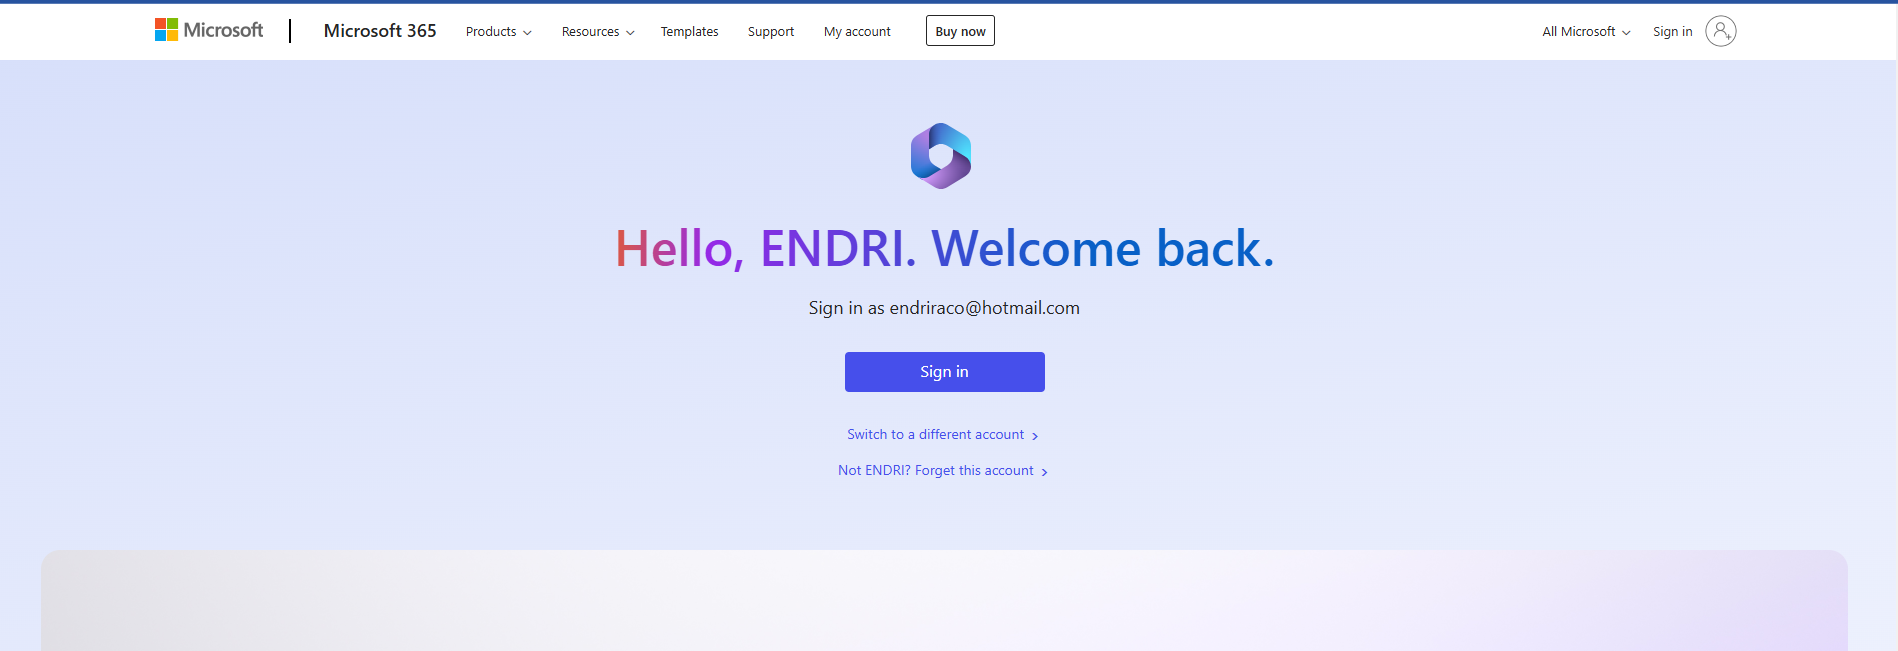
\includegraphics{./images/outlook1.png}
\end{frame}

\begin{frame}{Hapi 2: Futja e kredencialeve}
\phantomsection\label{hapi-2-futja-e-kredencialeve}
\begin{enumerate}
\item
  Shkruani adresën tuaj të email-it (p.sh.,
  \textbf{\href{mailto:emri.juaj@domain.com}{\nolinkurl{emri.juaj@domain.com}}}).
\item
  Klikoni \textbf{``Next''} (Vazhdo).
\end{enumerate}
\end{frame}

\begin{frame}{Hapi 2: Futja e kredencialeve}
\phantomsection\label{hapi-2-futja-e-kredencialeve-1}
\begin{enumerate}
\setcounter{enumi}{2}
\tightlist
\item
  Vendosni fjalëkalimin dhe klikoni \textbf{``Sign In''}.
\end{enumerate}

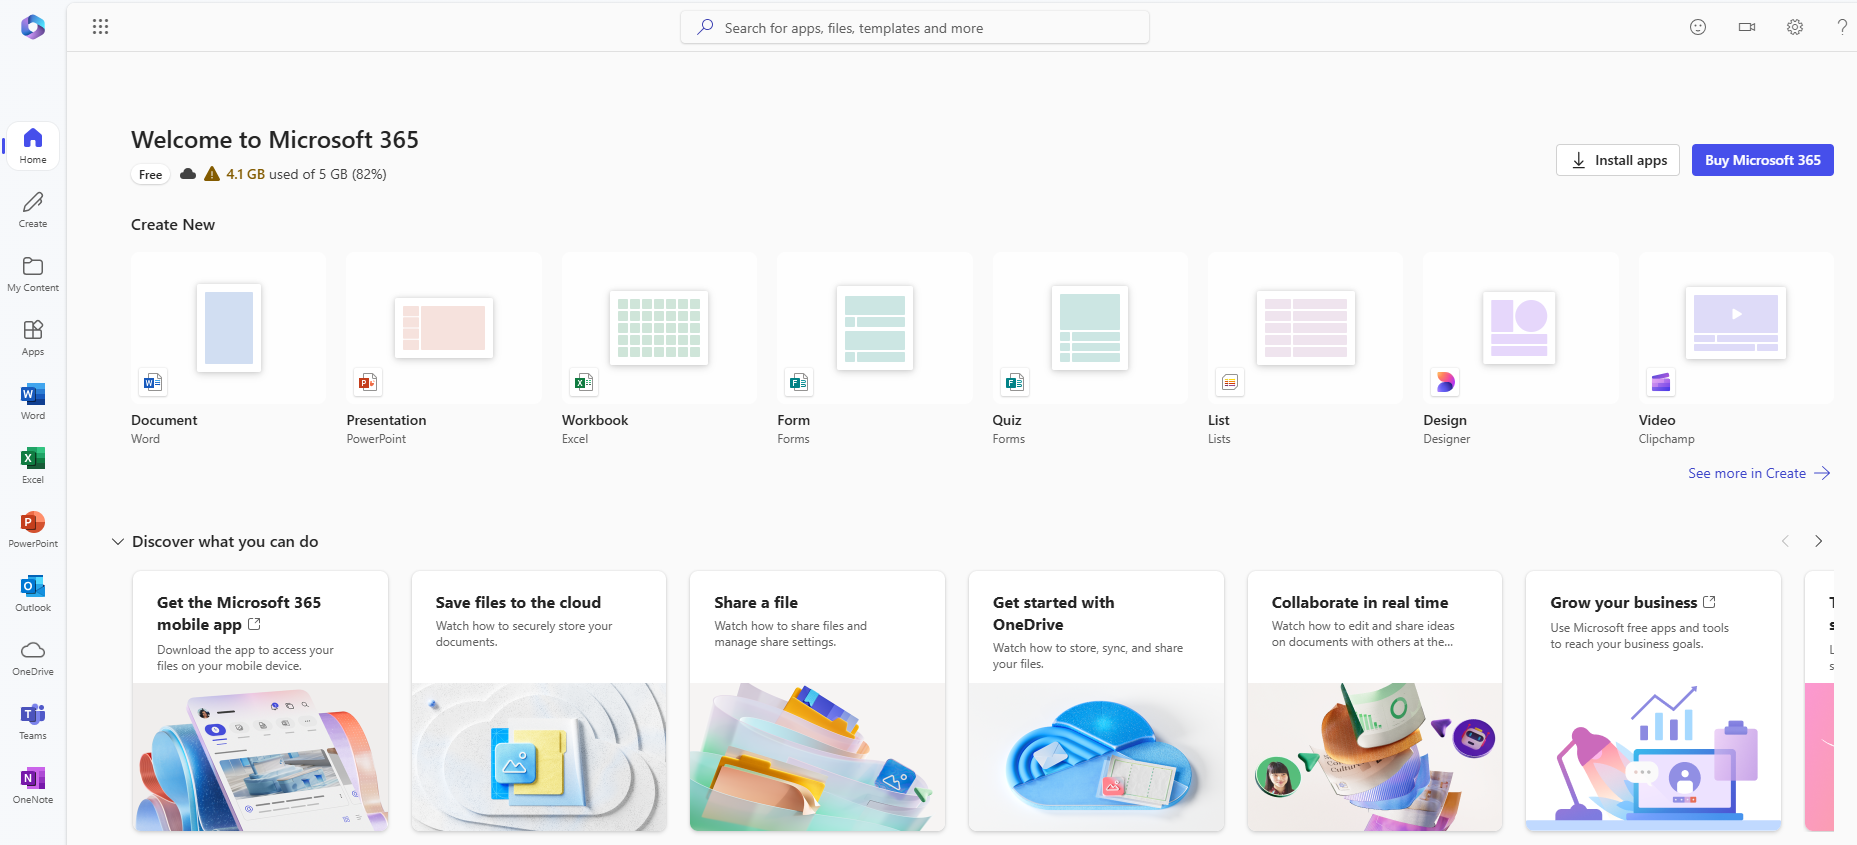
\includegraphics{./images/outlook2.png}
\end{frame}

\section{Outlook 365 Web}\label{outlook-365-web}

\begin{frame}{Hapi 3: Hyrja në Outlook}
\phantomsection\label{hapi-3-hyrja-nuxeb-outlook}
\begin{enumerate}
\tightlist
\item
  Pasi të hyni në \textbf{Office 365}, do të shfaqet paneli kryesor.
\end{enumerate}
\end{frame}

\begin{frame}{Hapi 3: Hyrja në Outlook}
\phantomsection\label{hapi-3-hyrja-nuxeb-outlook-1}
\begin{enumerate}
\setcounter{enumi}{1}
\tightlist
\item
  Klikoni ikonën \textbf{Outlook}.

  \begin{itemize}
  \tightlist
  \item
    Ikona duket si një zarf i kaltër.
  \end{itemize}
\end{enumerate}

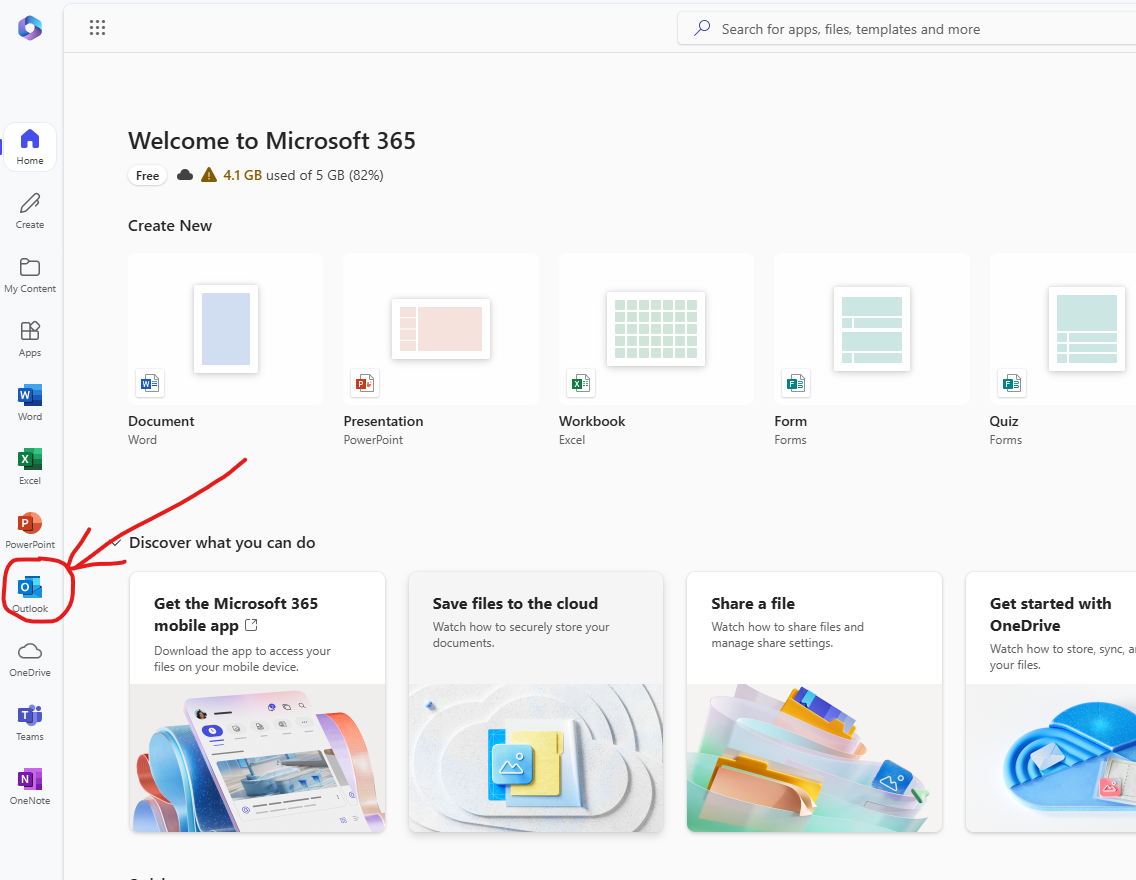
\includegraphics{./images/outlook3.png}
\end{frame}

\begin{frame}{Hapi 4: Njohja me ndërfaqen e Outlook Web}
\phantomsection\label{hapi-4-njohja-me-nduxebrfaqen-e-outlook-web}
\begin{itemize}
\item
  \textbf{Inbox}: Email-et që keni marrë.
\item
  \textbf{New Email}: Për të krijuar dhe dërguar një email të ri.
\item
  \textbf{Folders}: Dosje për të organizuar emailet.
\end{itemize}
\end{frame}

\begin{frame}{Hapi 4: Njohja me ndërfaqen e Outlook Web}
\phantomsection\label{hapi-4-njohja-me-nduxebrfaqen-e-outlook-web-1}
\begin{itemize}
\tightlist
\item
  \textbf{Search}: Për të kërkuar email-et sipas emrit ose përmbajtjes.
\end{itemize}

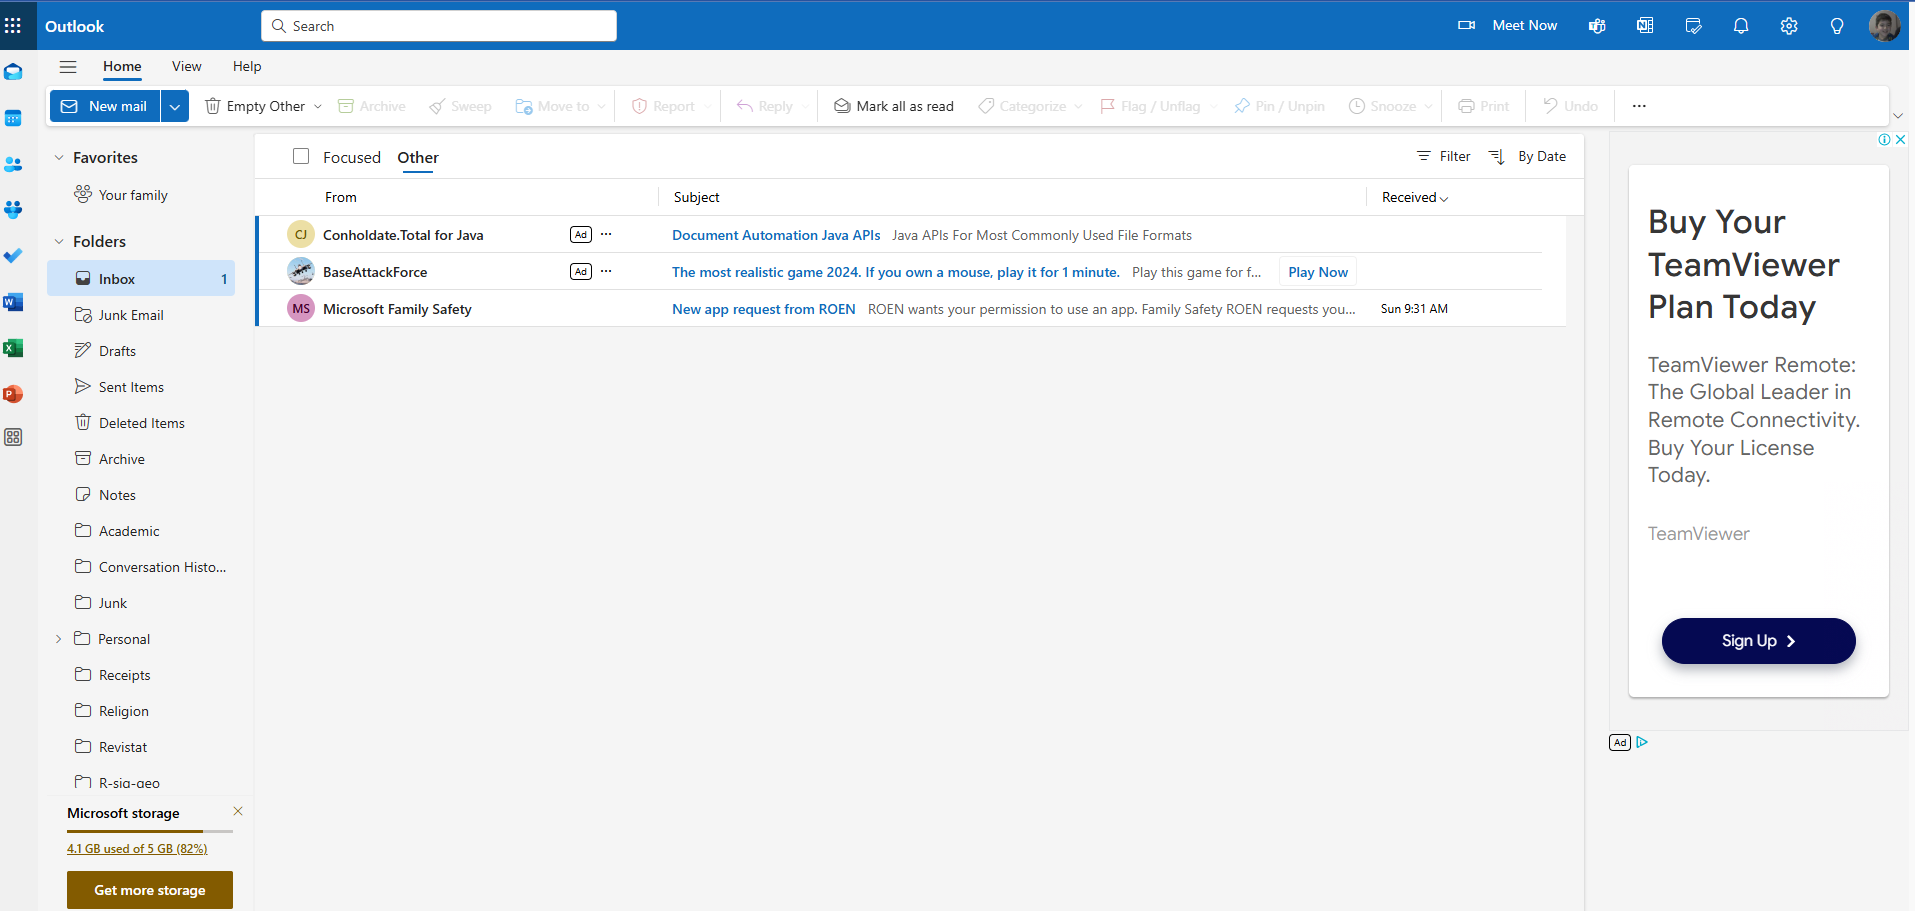
\includegraphics{./images/outlook4.png}
\end{frame}

\begin{frame}{Hapi 5: Dërgimi i një email-i të ri}
\phantomsection\label{hapi-5-duxebrgimi-i-njuxeb-email-i-tuxeb-ri}
\begin{enumerate}
\item
  Klikoni butonin \textbf{``New Email''} (Email i Ri).
\item
  Plotësoni fushat:

  \begin{itemize}
  \item
    \textbf{To}: Adresa e marrësit.
  \item
    \textbf{Subject}: Subjekti i email-it.
  \item
    \textbf{Body}: Përmbajtja e email-it.
  \end{itemize}
\end{enumerate}
\end{frame}

\begin{frame}{Hapi 5: Dërgimi i një email-i të ri}
\phantomsection\label{hapi-5-duxebrgimi-i-njuxeb-email-i-tuxeb-ri-1}
\begin{enumerate}
\setcounter{enumi}{2}
\tightlist
\item
  Klikoni \textbf{``Send''} (Dërgo).
\end{enumerate}

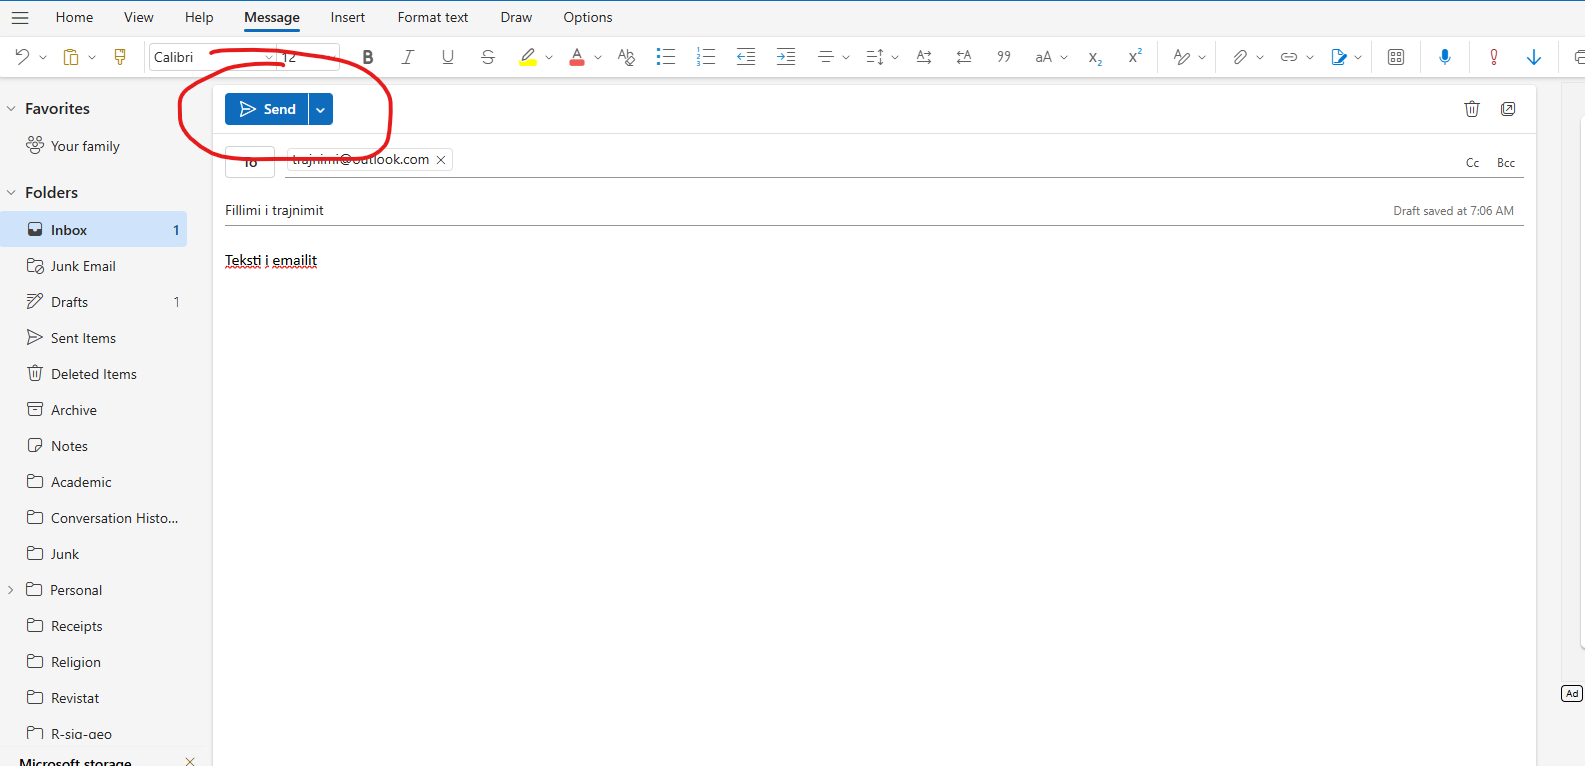
\includegraphics{./images/outlook5.png}
\end{frame}

\begin{frame}{Hapi 6: Kontrollimi i mesazheve}
\phantomsection\label{hapi-6-kontrollimi-i-mesazheve}
\begin{itemize}
\item
  \textbf{Unread}: Mesazhet e pa lexuara shfaqen me ngjyrë më të errët.
\item
  Klikoni mbi email-in për ta hapur.
\end{itemize}
\end{frame}

\begin{frame}{Hapi 6: Kontrollimi i mesazheve}
\phantomsection\label{hapi-6-kontrollimi-i-mesazheve-1}
\begin{itemize}
\tightlist
\item
  Përgjigjuni ose dërgoni përpara email-in duke përdorur komandat në
  krye.
\end{itemize}

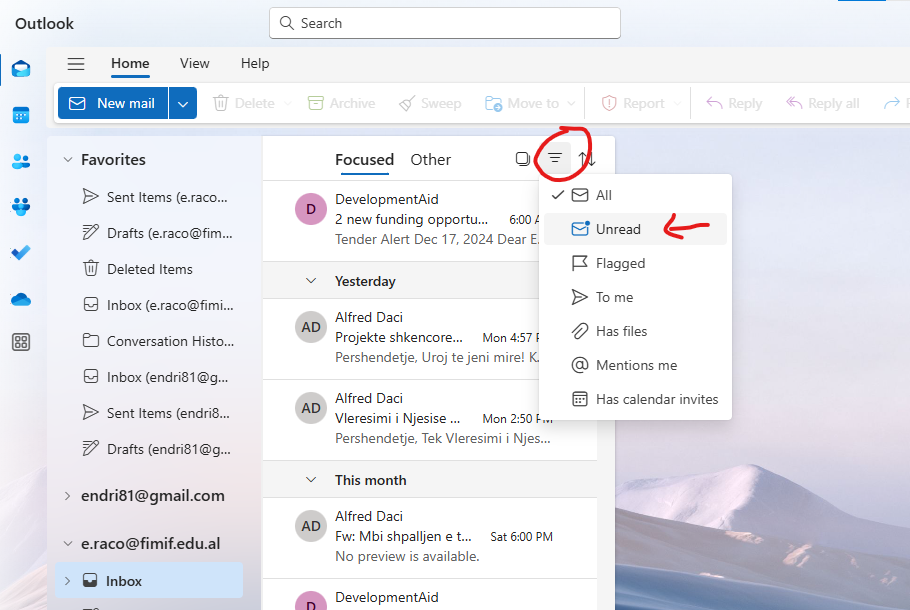
\includegraphics{./images/outlook6.png}
\end{frame}

\begin{frame}{Rezultati}
\phantomsection\label{rezultati}
\begin{itemize}
\item
  Tani mund të përdorni \textbf{Outlook 365 Web} për:

  \begin{itemize}
  \item
    Të lexoni dhe dërgoni email-e.
  \item
    Të organizoni emailet në dosje.
  \item
    Të bashkëpunoni lehtësisht në kohë reale.
  \end{itemize}
\end{itemize}
\end{frame}

\begin{frame}{Pyetje \& Diskutim}
\phantomsection\label{pyetje-diskutim-1}
\begin{itemize}
\tightlist
\item
  A kishte ndonjë hap që ju u duk i paqartë?
\end{itemize}
\end{frame}

\begin{frame}{Nënshkrimi në email}
\phantomsection\label{nuxebnshkrimi-nuxeb-email}
\begin{itemize}
\item
  \textbf{Nënshkrimi në email} përmban informacionin tuaj personal dhe
  profesional, si:

  \begin{itemize}
  \item
    Emri dhe mbiemri
  \item
    Pozicioni juaj në organizatë
  \item
    Informacion kontakti (numër telefoni, adresë email-i)
  \end{itemize}
\end{itemize}
\end{frame}

\begin{frame}{Nënshkrimi në email}
\phantomsection\label{nuxebnshkrimi-nuxeb-email-1}
\begin{itemize}
\tightlist
\item
  \textbf{Përdorimi i nënshkrimit} tregon profesionalizëm dhe kursen
  kohë për çdo email që dërgoni.
\end{itemize}
\end{frame}

\begin{frame}{Hapi 1: Hyrja në cilësimet (Settings)}
\phantomsection\label{hapi-1-hyrja-nuxeb-ciluxebsimet-settings}
\begin{enumerate}
\item
  Klikoni mbi \textbf{ikonën e ingranazhit} \(\bigodot\) në këndin e
  sipërm të djathtë.
\item
  Në panelin anësor, klikoni në fund mbi \textbf{``Account''}.
\end{enumerate}

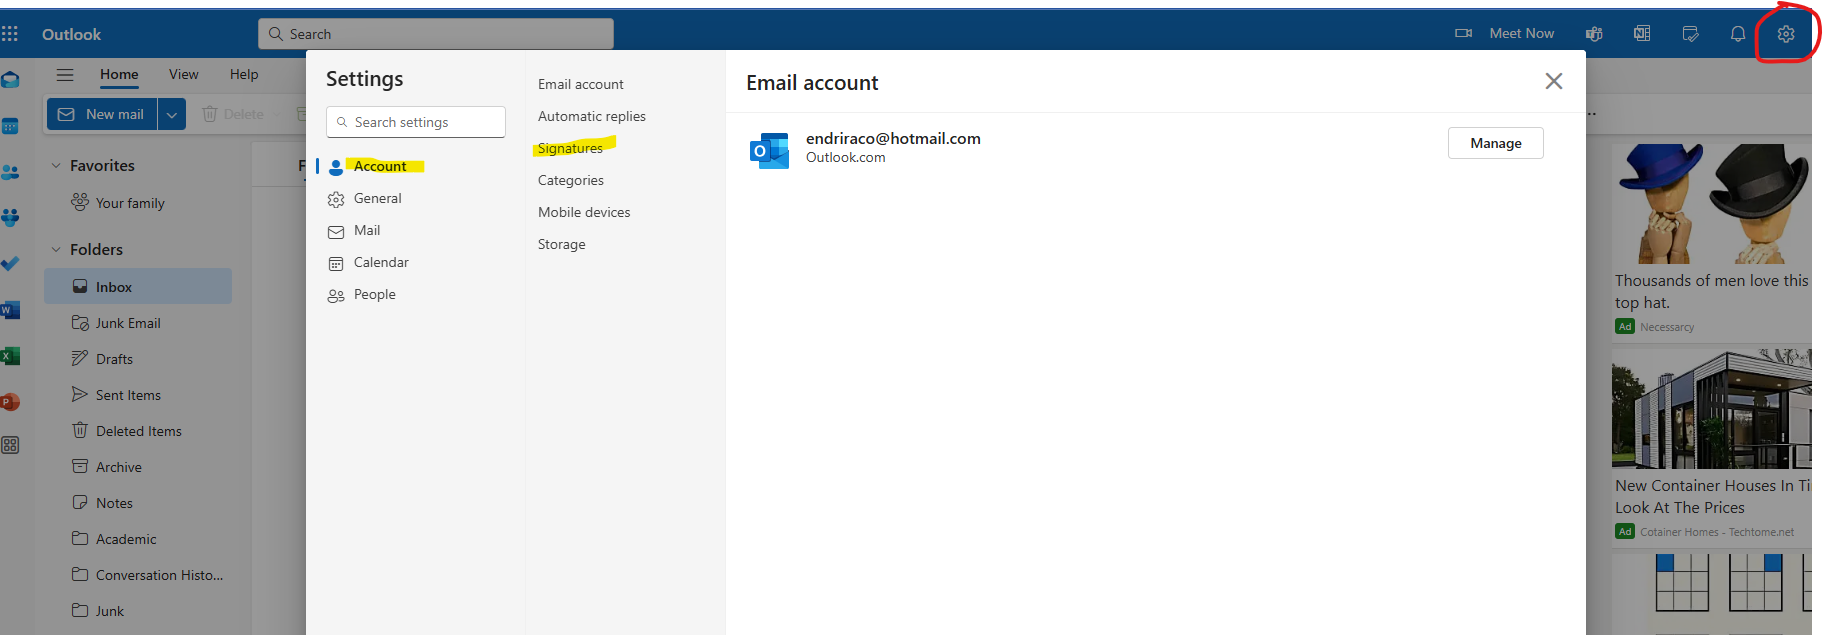
\includegraphics{./images/outlook7.png}
\end{frame}

\begin{frame}{Hapi 2: Gjetja e opsionit për nënshkrim}
\phantomsection\label{hapi-2-gjetja-e-opsionit-puxebr-nuxebnshkrim}
\begin{enumerate}
\tightlist
\item
  Nga dritarja e cilësimeve, zgjidhni \textbf{Signatures}
\end{enumerate}

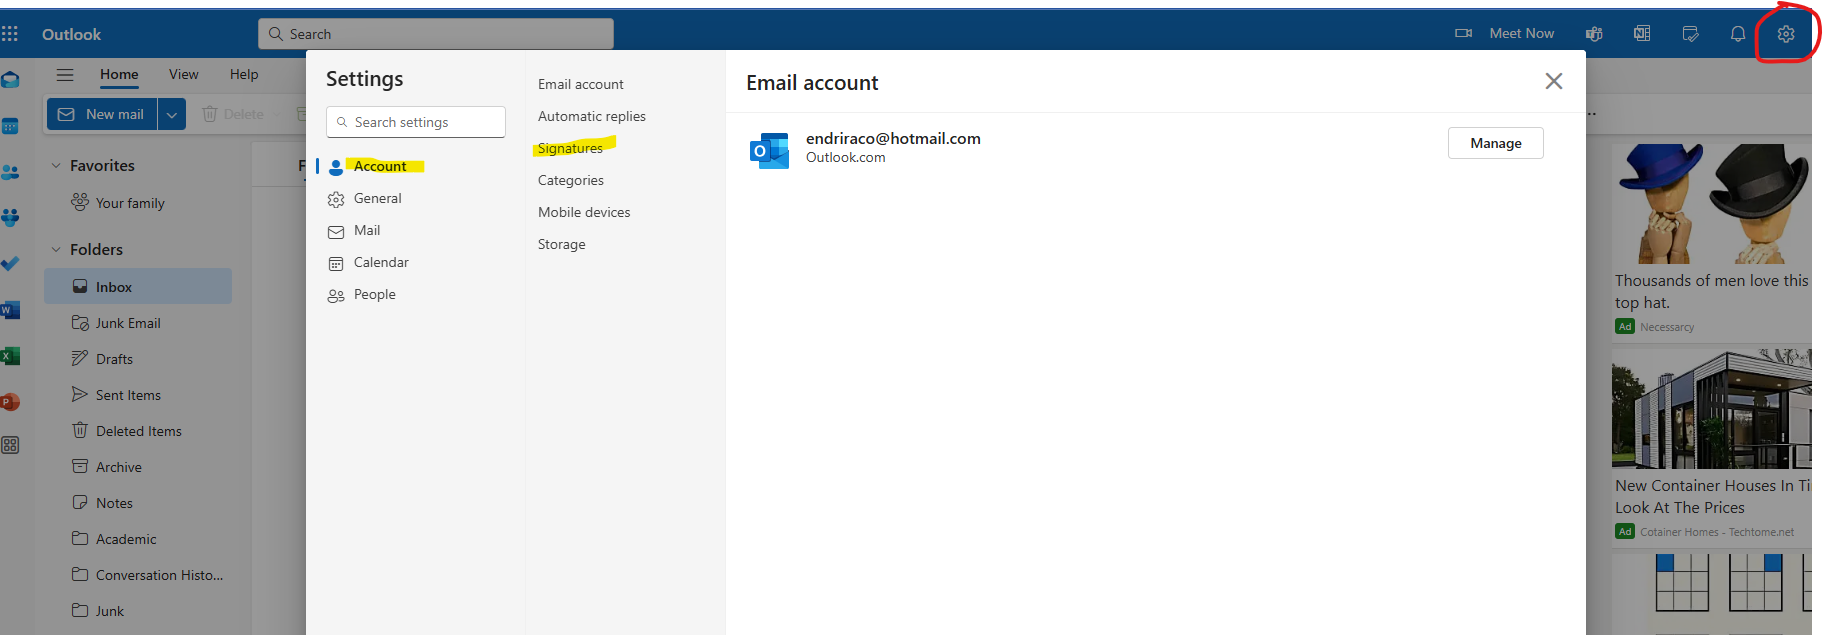
\includegraphics{./images/outlook7.png}
\end{frame}

\begin{frame}{Hapi 3: Krijimi i nënshkrimit}
\phantomsection\label{hapi-3-krijimi-i-nuxebnshkrimit}
\begin{enumerate}
\item
  Në kutinë për tekst, shkruani nënshkrimin tuaj:

  \begin{itemize}
  \item
    \textbf{Emri juaj}
  \item
    \textbf{Pozicioni juaj}
  \item
    \textbf{Informacion kontakti}
  \end{itemize}
\end{enumerate}
\end{frame}

\begin{frame}{Hapi 3: Krijimi i nënshkrimit}
\phantomsection\label{hapi-3-krijimi-i-nuxebnshkrimit-1}
\begin{enumerate}
\setcounter{enumi}{1}
\item
  Opsionale: Përdorni opsionet për të formatuar tekstin (bold, italic,
  font).
\item
  Mund të shtoni edhe një \textbf{logo} ose një \textbf{link}.
\end{enumerate}

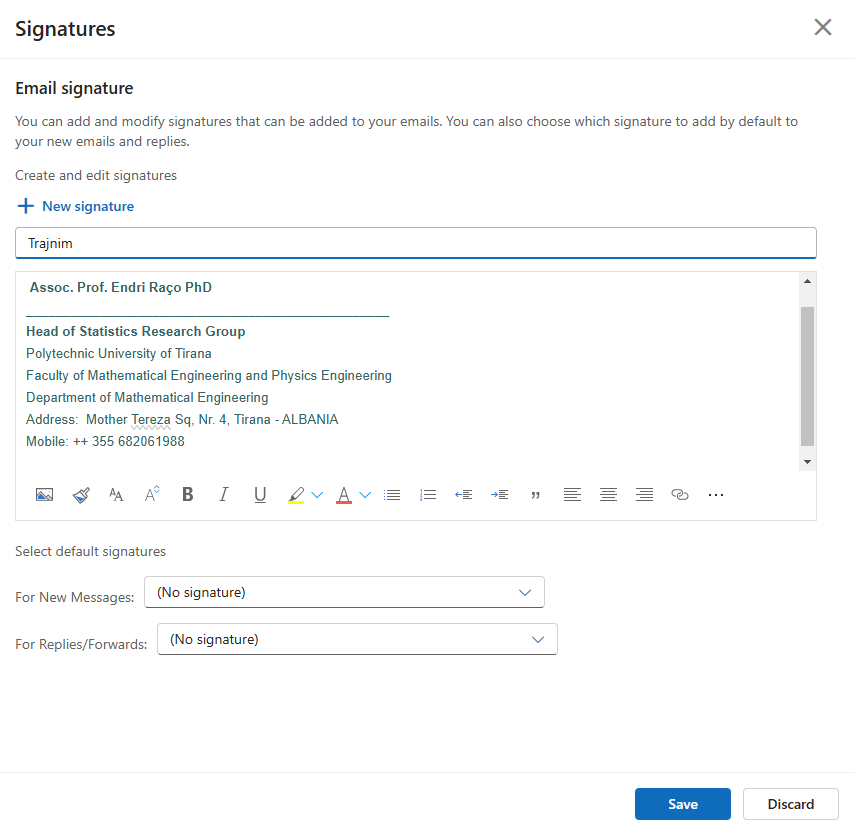
\includegraphics{./images/outlook8.png}
\end{frame}

\begin{frame}{Hapi 4: Aplikimi i nënshkrimit në email-et tuaja}
\phantomsection\label{hapi-4-aplikimi-i-nuxebnshkrimit-nuxeb-email-et-tuaja}
\begin{enumerate}
\item
  Poshtë kutisë së nënshkrimit, zgjidhni:

  \begin{itemize}
  \item
    \textbf{Automatically include my signature on new messages} (Për
    email të rinj).
  \item
    \textbf{Automatically include my signature on messages I forward or
    reply to} (Për përgjigje ose përcjellje).
  \end{itemize}
\end{enumerate}

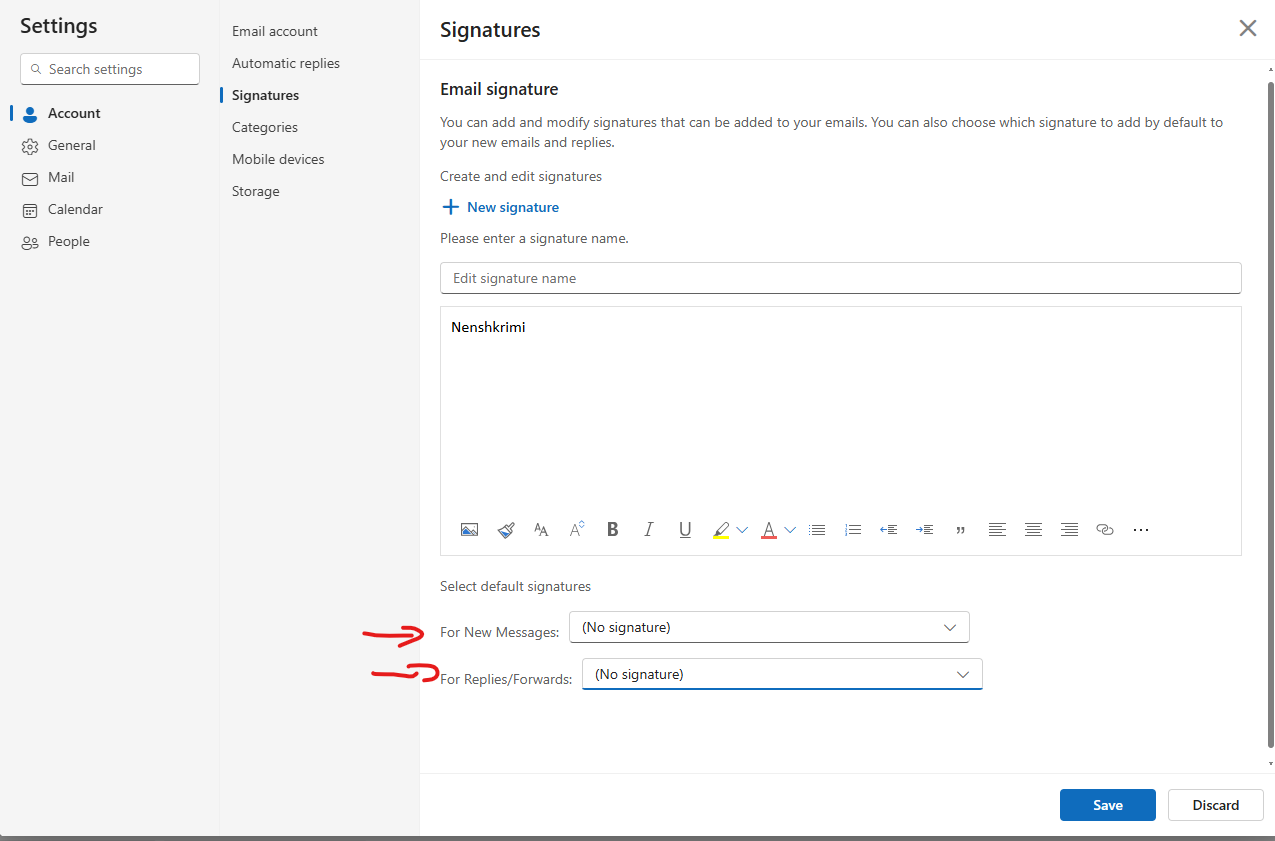
\includegraphics{./images/outlook9.png}
\end{frame}

\begin{frame}{Hapi 4: Aplikimi i nënshkrimit në email-et tuaja}
\phantomsection\label{hapi-4-aplikimi-i-nuxebnshkrimit-nuxeb-email-et-tuaja-1}
\begin{enumerate}
\setcounter{enumi}{1}
\tightlist
\item
  Klikoni \textbf{Save} (Ruaj) për të aplikuar ndryshimet.
\end{enumerate}
\end{frame}

\begin{frame}{Hapi 5: Testimi i nënshkrimit}
\phantomsection\label{hapi-5-testimi-i-nuxebnshkrimit}
\begin{enumerate}
\item
  Krijoni një email të ri duke klikuar mbi \textbf{``New Email''}.
\item
  Kontrolloni nëse nënshkrimi shfaqet automatikisht në fund të email-it.
\end{enumerate}

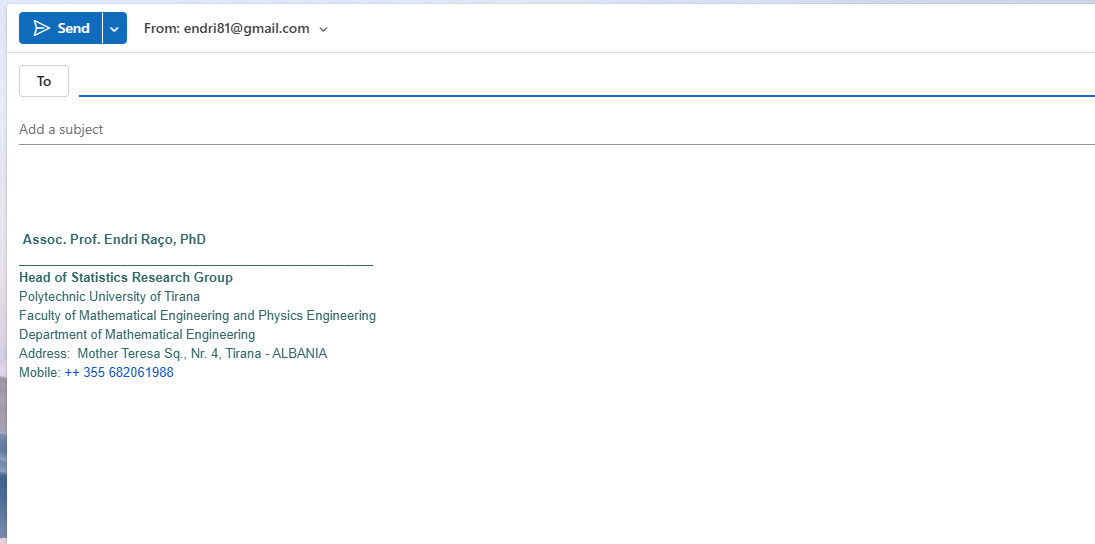
\includegraphics{./images/outlook10.png}
\end{frame}

\begin{frame}{Rezultat}
\phantomsection\label{rezultat}
\begin{itemize}
\item
  Tani nënshkrimi juaj shfaqet automatikisht në çdo email.
\item
  Mund të përditësoni ose ndryshoni nënshkrimin në çdo moment përmes
  cilësimeve të Outlook.
\end{itemize}
\end{frame}

\begin{frame}{Rezultat}
\phantomsection\label{rezultat-1}
\begin{itemize}
\item
  A keni hasur ndonjë vështirësi gjatë konfigurimit të nënshkrimit?
\item
  Çfarë elementi tjetër mund të shtoni në nënshkrimin tuaj për ta bërë
  më profesional?
\end{itemize}
\end{frame}

\begin{frame}{Inbox i organizuar}
\phantomsection\label{inbox-i-organizuar}
\begin{itemize}
\item
  Një \textbf{Inbox i organizuar} ju ndihmon të:

  \begin{itemize}
  \item
    Gjeni email-et më shpejt.
  \item
    Ruani emailet sipas projekteve ose prioriteteve.
  \item
    Rrisni produktivitetin dhe efikasitetin tuaj në komunikim.
  \end{itemize}
\item
  \textbf{Outlook 365 Web} ofron opsionin për të krijuar dhe menaxhuar
  \textbf{dosje (folders)} lehtësisht.
\end{itemize}
\end{frame}

\begin{frame}{Hapi 1: Gjetja e seksionit të dosjeve}
\phantomsection\label{hapi-1-gjetja-e-seksionit-tuxeb-dosjeve}
\begin{enumerate}
\tightlist
\item
  Në panelin e majtë të ekranit, do të shihni listën e dosjeve:
\end{enumerate}

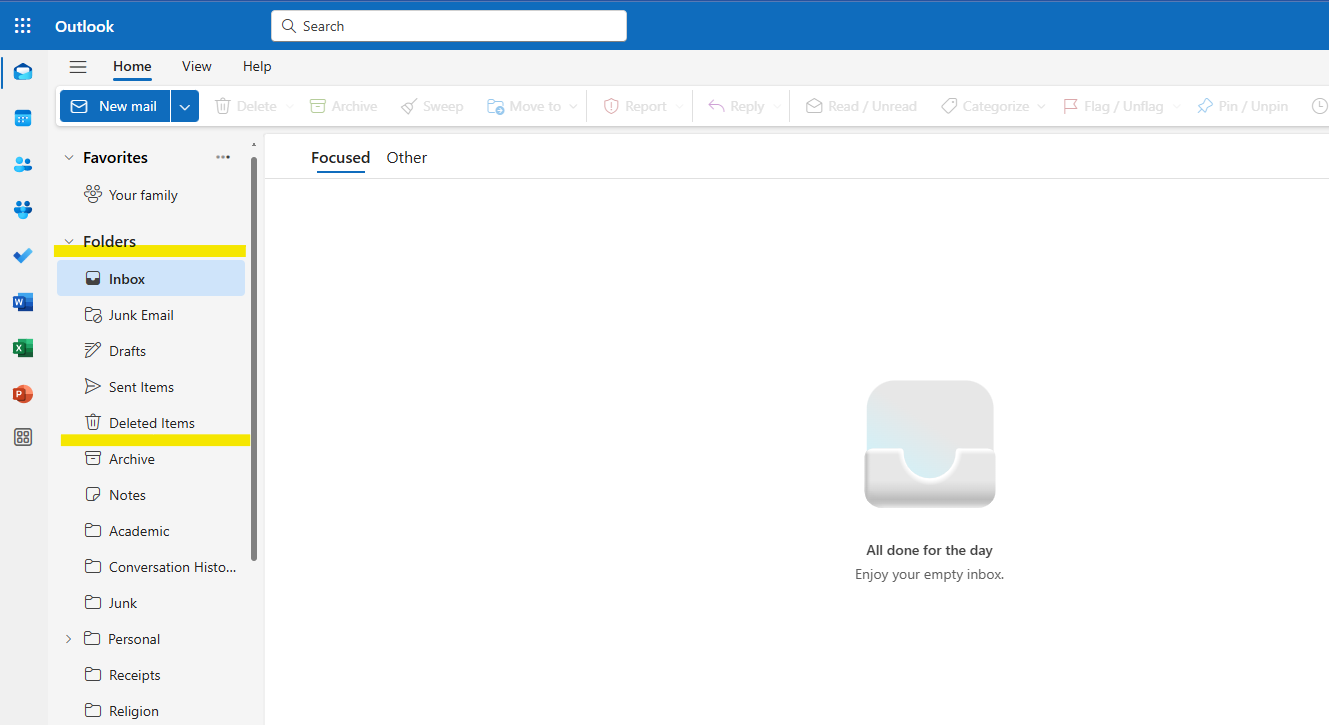
\includegraphics{./images/outlook11.png}
\end{frame}

\begin{frame}{Hapi 1: Gjetja e seksionit të dosjeve}
\phantomsection\label{hapi-1-gjetja-e-seksionit-tuxeb-dosjeve-1}
\begin{itemize}
\item
  \textbf{Inbox}: Email-et e ardhura.
\item
  \textbf{Drafts}: Email-et e ruajtura si draft.
\end{itemize}
\end{frame}

\begin{frame}{Hapi 1: Gjetja e seksionit të dosjeve}
\phantomsection\label{hapi-1-gjetja-e-seksionit-tuxeb-dosjeve-2}
\begin{itemize}
\item
  \textbf{Sent Items}: Email-et e dërguara.
\item
  \textbf{Deleted Items}: Email-et e fshira.
\end{itemize}
\end{frame}

\begin{frame}{Hapi 1: Gjetja e seksionit të dosjeve}
\phantomsection\label{hapi-1-gjetja-e-seksionit-tuxeb-dosjeve-3}
\begin{enumerate}
\setcounter{enumi}{1}
\item
  Afroni kursorin tek \textbf{Folders} ose tek dosjet \textbf{Inbox} etj
\item
  Do shfaqen 3 pika me opsionin për \textbf{krijimin e dosjeve të reja}.
\end{enumerate}

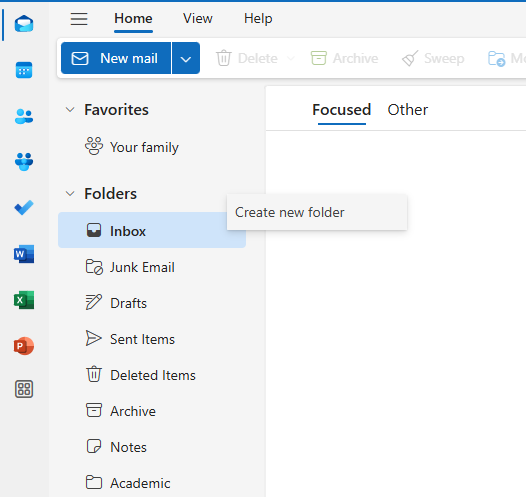
\includegraphics{./images/outlook12.png}
\end{frame}

\begin{frame}{Hapi 2: Krijimi i një dosjeje të re}
\phantomsection\label{hapi-2-krijimi-i-njuxeb-dosjeje-tuxeb-re}
\begin{enumerate}
\item
  Klikoni me të djathtën mbi \textbf{Inbox} ose në ndonjë seksion
  tjetër.
\item
  Zgjidhni \textbf{``Create New Folder''} (Krijo një Dosje të Re).
\end{enumerate}
\end{frame}

\begin{frame}{Hapi 2: Krijimi i një dosjeje të re}
\phantomsection\label{hapi-2-krijimi-i-njuxeb-dosjeje-tuxeb-re-1}
\begin{enumerate}
\setcounter{enumi}{2}
\item
  Jepni emrin e dosjes, p.sh., \textbf{``Projekti A''} ose
  \textbf{``Prioritetet''}.
\item
  Shtypni \textbf{Enter} për ta ruajtur dosjen.
\end{enumerate}

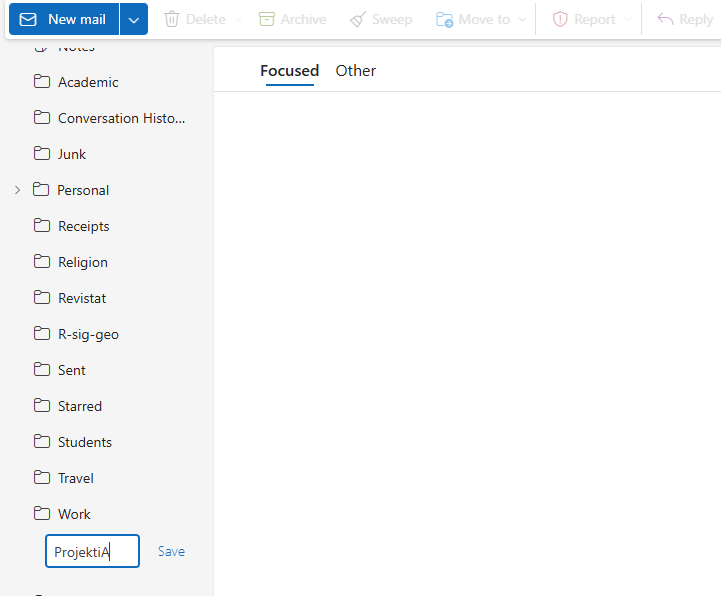
\includegraphics{./images/outlook13.png}
\end{frame}

\begin{frame}{Hapi 3: Zhvendosja e emaileve në dosje}
\phantomsection\label{hapi-3-zhvendosja-e-emaileve-nuxeb-dosje}
\begin{enumerate}
\item
  Klikoni me të djathtën mbi email-in që dëshironi të zhvendosni.
\item
  Zgjidhni \textbf{``Move''} (Zhvendos) dhe pastaj zgjidhni dosjen ku
  dëshironi ta ruani email-in.
\end{enumerate}
\end{frame}

\begin{frame}{Hapi 3: Zhvendosja e emaileve në dosje}
\phantomsection\label{hapi-3-zhvendosja-e-emaileve-nuxeb-dosje-1}
\begin{itemize}
\tightlist
\item
  Alternativë: \textbf{Drag \& Drop} -- tërhiqni email-in dhe lëshojeni
  në dosjen përkatëse.
\end{itemize}

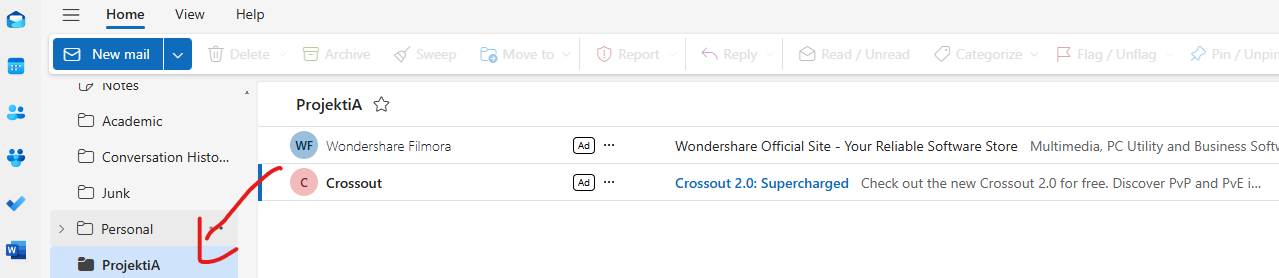
\includegraphics{./images/outlook14.png}
\end{frame}

\begin{frame}{Hapi 4: Krijimi i sub-dosjeve për organizim më të mirë}
\phantomsection\label{hapi-4-krijimi-i-sub-dosjeve-puxebr-organizim-muxeb-tuxeb-miruxeb}
\begin{enumerate}
\item
  Klikoni me të djathtën mbi një dosje ekzistuese.
\item
  Zgjidhni \textbf{``Create New Subfolder''} (Krijo Nëndosje).
\end{enumerate}
\end{frame}

\begin{frame}{Hapi 4: Krijimi i sub-dosjeve për organizim më të mirë}
\phantomsection\label{hapi-4-krijimi-i-sub-dosjeve-puxebr-organizim-muxeb-tuxeb-miruxeb-1}
\begin{enumerate}
\setcounter{enumi}{2}
\tightlist
\item
  Emërtoni sub-dosjen sipas nevojës, p.sh., \textbf{``Email-e të
  Marrësve''}.
\end{enumerate}

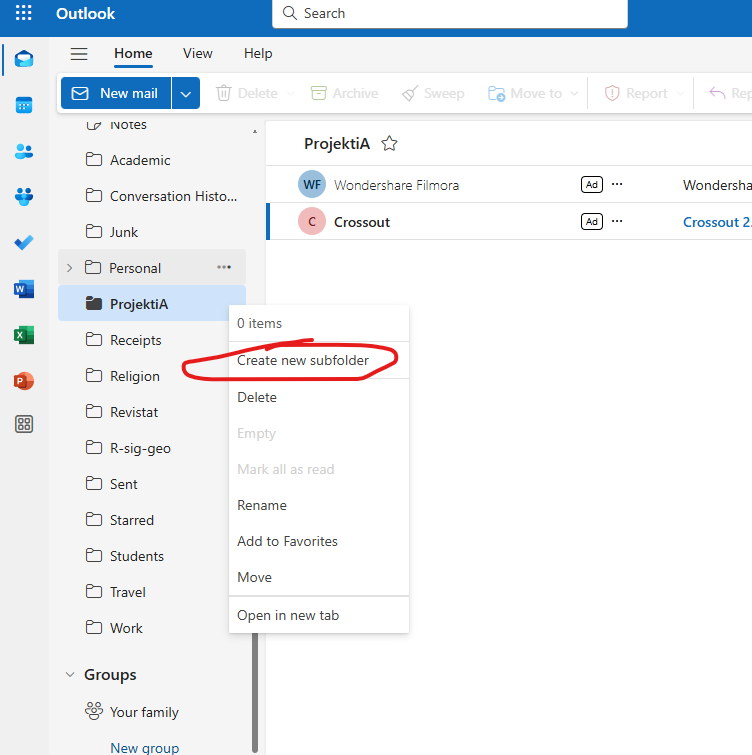
\includegraphics{./images/outlook15.png}
\end{frame}

\begin{frame}{Hapi 5: Rregulli për organizim automatik}
\phantomsection\label{hapi-5-rregulli-puxebr-organizim-automatik}
\begin{enumerate}
\tightlist
\item
  Klikoni \textbf{Settings} dhe zgjidhni nga \textbf{Mails} opsionin
  \textbf{``Rules''} (Krijo Rregull).
\end{enumerate}

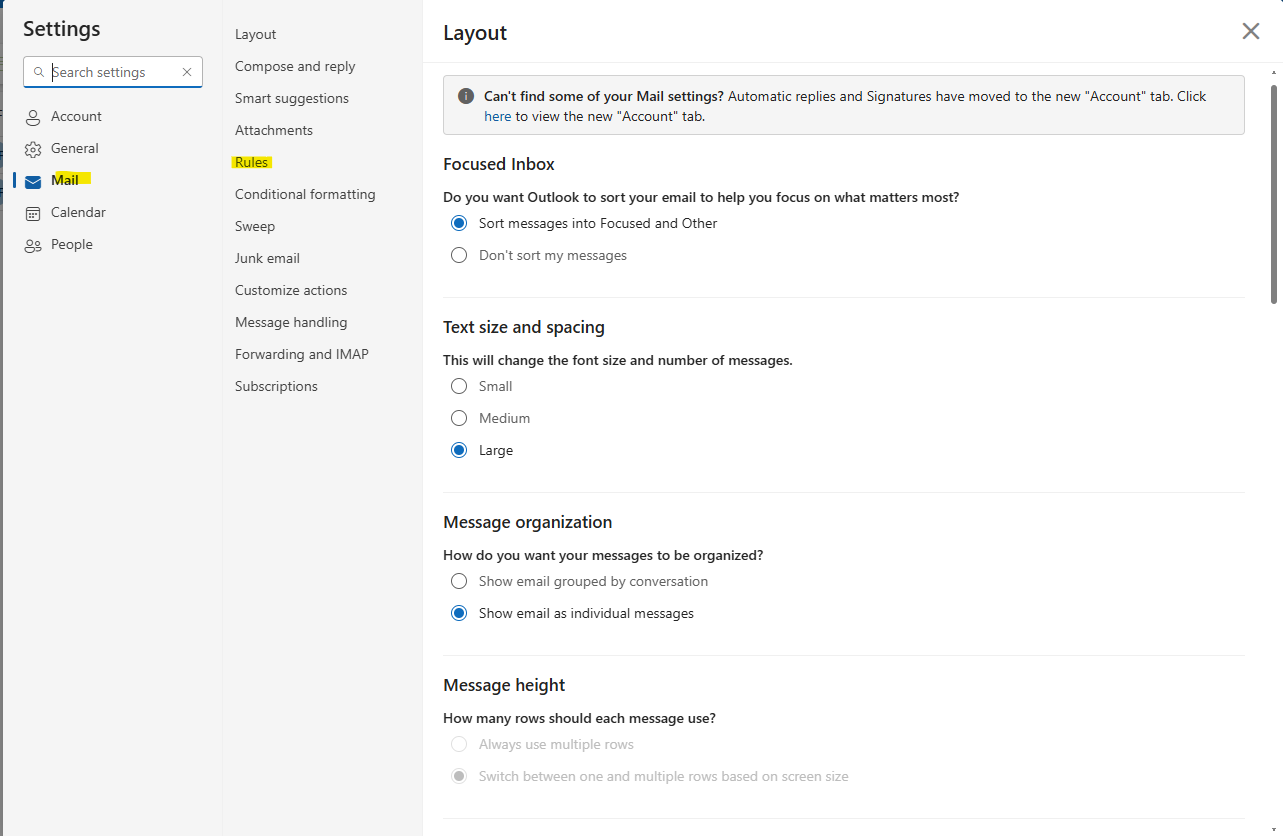
\includegraphics{./images/outlook16.png}
\end{frame}

\begin{frame}{Hapi 5: Rregulli për organizim automatik}
\phantomsection\label{hapi-5-rregulli-puxebr-organizim-automatik-1}
\begin{enumerate}
\setcounter{enumi}{1}
\item
  Vendosni rregulla për zhvendosjen automatike të email-eve në një dosje
  bazuar në:

  \begin{itemize}
  \item
    \textbf{Dërguesin}
  \item
    \textbf{Subjektin}
  \item
    \textbf{Fjalë kyçe}
  \end{itemize}
\end{enumerate}
\end{frame}

\begin{frame}{Hapi 5: Rregulli për organizim automatik}
\phantomsection\label{hapi-5-rregulli-puxebr-organizim-automatik-2}
\begin{enumerate}
\setcounter{enumi}{2}
\tightlist
\item
  Ruani rregullin dhe testoni funksionimin e tij.
\end{enumerate}
\end{frame}

\begin{frame}{Përfitimet e organizimit me dosje}
\phantomsection\label{puxebrfitimet-e-organizimit-me-dosje}
\begin{itemize}
\item
  \textbf{Efikasitet}: Gjeni emailet më lehtë dhe më shpejt.
\item
  \textbf{Prioritizim}: Ruani email-et sipas rëndësisë dhe temës.
\item
  \textbf{Automatizim}: Zhvendosni email-et automatikisht me rregullat e
  vendosura.
\end{itemize}
\end{frame}

\begin{frame}{Rezultati}
\phantomsection\label{rezultati-1}
\begin{itemize}
\item
  Krijimi dhe menaxhimi i \textbf{dosjeve} në Outlook Web është një
  mënyrë efektive për të mbajtur inbox-in të organizuar.
\item
  Përdorni funksionet si \textbf{sub-dosjet} dhe \textbf{rregullat} për
  të kursyer kohë dhe për të përmirësuar produktivitetin tuaj.
\end{itemize}
\end{frame}

\begin{frame}{Pyetje \& Diskutim}
\phantomsection\label{pyetje-diskutim-2}
\begin{itemize}
\tightlist
\item
  A kishit përdorur më parë funksionin e dosjeve në Outlook?
\end{itemize}
\end{frame}

\begin{frame}{Funksioni i kërkimit}
\phantomsection\label{funksioni-i-kuxebrkimit}
\begin{itemize}
\item
  \textbf{Funksioni i kërkimit} në \textbf{Outlook 365 Web} ju ndihmon
  të:

  \begin{itemize}
  \item
    Gjeni emailet specifike në mënyrë të shpejtë.
  \item
    Filtroni mesazhet sipas dërguesit, subjektit ose fjalëve kyçe.
  \item
    Kursejnë kohë dhe përmirësoni efikasitetin tuaj.
  \end{itemize}
\end{itemize}
\end{frame}

\begin{frame}{Hapi 1: Gjetja e shiritit të kërkimit}
\phantomsection\label{hapi-1-gjetja-e-shiritit-tuxeb-kuxebrkimit}
\begin{enumerate}
\item
  Shiriti i kërkimit gjendet në \textbf{krye të faqes} në Outlook Web.
\item
  Klikoni në kutinë e kërkimit ku shkruhet \textbf{``Search''} (Kërko).
\end{enumerate}

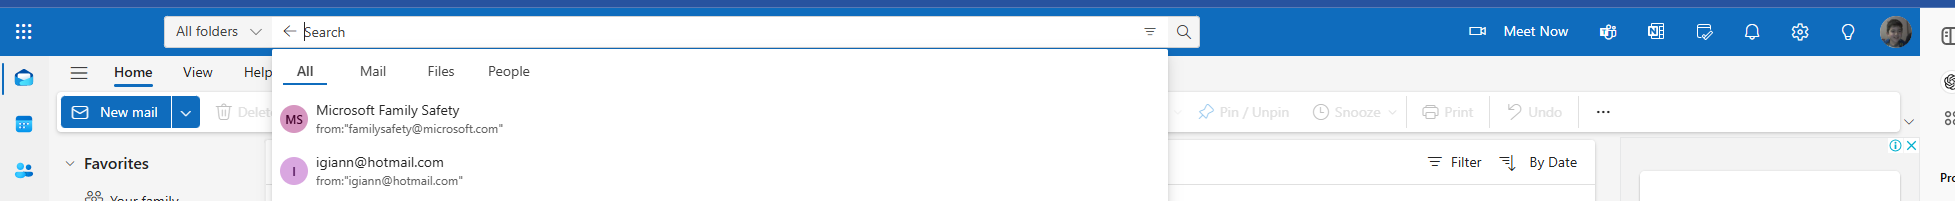
\includegraphics{./images/outlook18.png}
\end{frame}

\begin{frame}{Hapi 2: Kërkimi bazë}
\phantomsection\label{hapi-2-kuxebrkimi-bazuxeb}
\begin{enumerate}
\item
  Shkruani \textbf{një fjalë kyçe} ose \textbf{emrin e dërguesit} në
  kutinë e kërkimit.

  \begin{itemize}
  \tightlist
  \item
    P.sh., shkruani \textbf{``Endri Raço''} ose \textbf{``projekt''}.
  \end{itemize}
\item
  Klikoni \textbf{Enter} për të parë rezultatet.
\end{enumerate}
\end{frame}

\begin{frame}{Hapi 3: Filtrimi i rezultateve}
\phantomsection\label{hapi-3-filtrimi-i-rezultateve}
\begin{enumerate}
\item
  Pas kërkimit, Outlook ofron opsione për të filtruar rezultatet:

  \begin{itemize}
  \item
    \textbf{All}: Të gjitha emailet.
  \item
    \textbf{From}: Filtroni sipas dërguesit.
  \item
    \textbf{Subject}: Mesazhet që përmbajnë fjalë kyçe në subjekt.
  \item
    \textbf{Has attachments}: Filtroni mesazhet që kanë bashkëngjitje.
  \end{itemize}
\end{enumerate}
\end{frame}

\begin{frame}{Hapi 3: Filtrimi i rezultateve}
\phantomsection\label{hapi-3-filtrimi-i-rezultateve-1}
\begin{enumerate}
\setcounter{enumi}{1}
\tightlist
\item
  Zgjidhni filtrin e duhur për të ngushtuar kërkimin.
\end{enumerate}

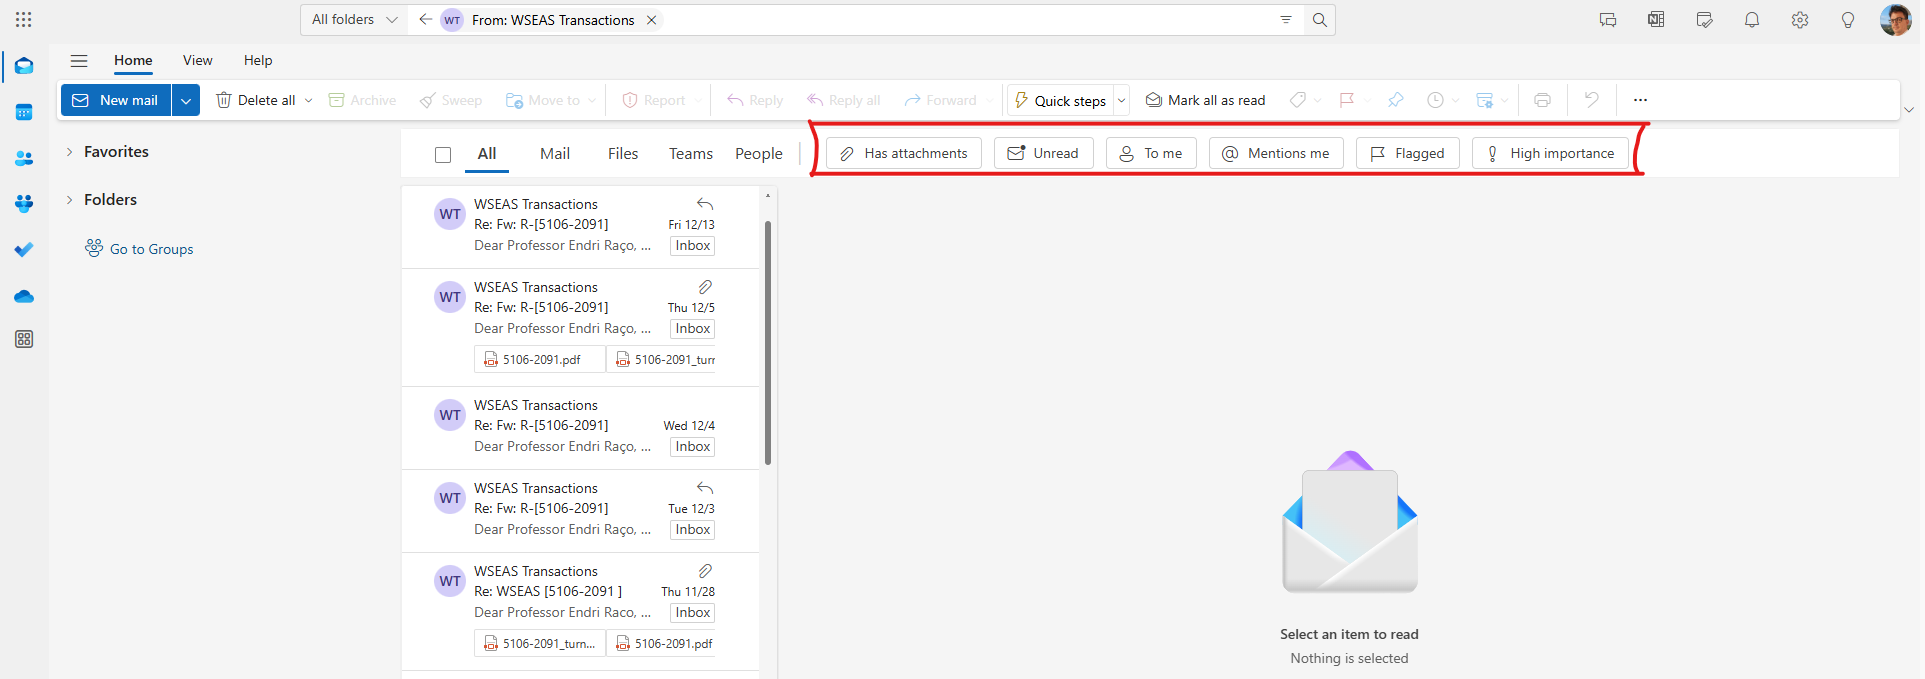
\includegraphics{./images/outlook19.png}
\end{frame}

\begin{frame}{Hapi 4: Kërkimi i avancuar}
\phantomsection\label{hapi-4-kuxebrkimi-i-avancuar}
\begin{enumerate}
\item
  Klikoni mbi \textbf{``Advanced Search''} ose përdorni filtrat
  manualisht:

  \begin{itemize}
  \item
    \textbf{From}: Dërguesi i email-it.
  \item
    \textbf{To}: Marrësi i email-it.
  \item
    \textbf{Subject}: Subjekti i email-it.
  \item
    \textbf{Date}: Filtroni sipas datës së dërgimit.
  \end{itemize}
\end{enumerate}
\end{frame}

\begin{frame}{Hapi 4: Kërkimi i avancuar}
\phantomsection\label{hapi-4-kuxebrkimi-i-avancuar-1}
\begin{enumerate}
\setcounter{enumi}{1}
\item
  Kombinoni filtrat për një kërkim më të saktë.

  \begin{itemize}
  \tightlist
  \item
    P.sh., \textbf{From: Endri Raço, Date: Last week}.
  \end{itemize}
\end{enumerate}

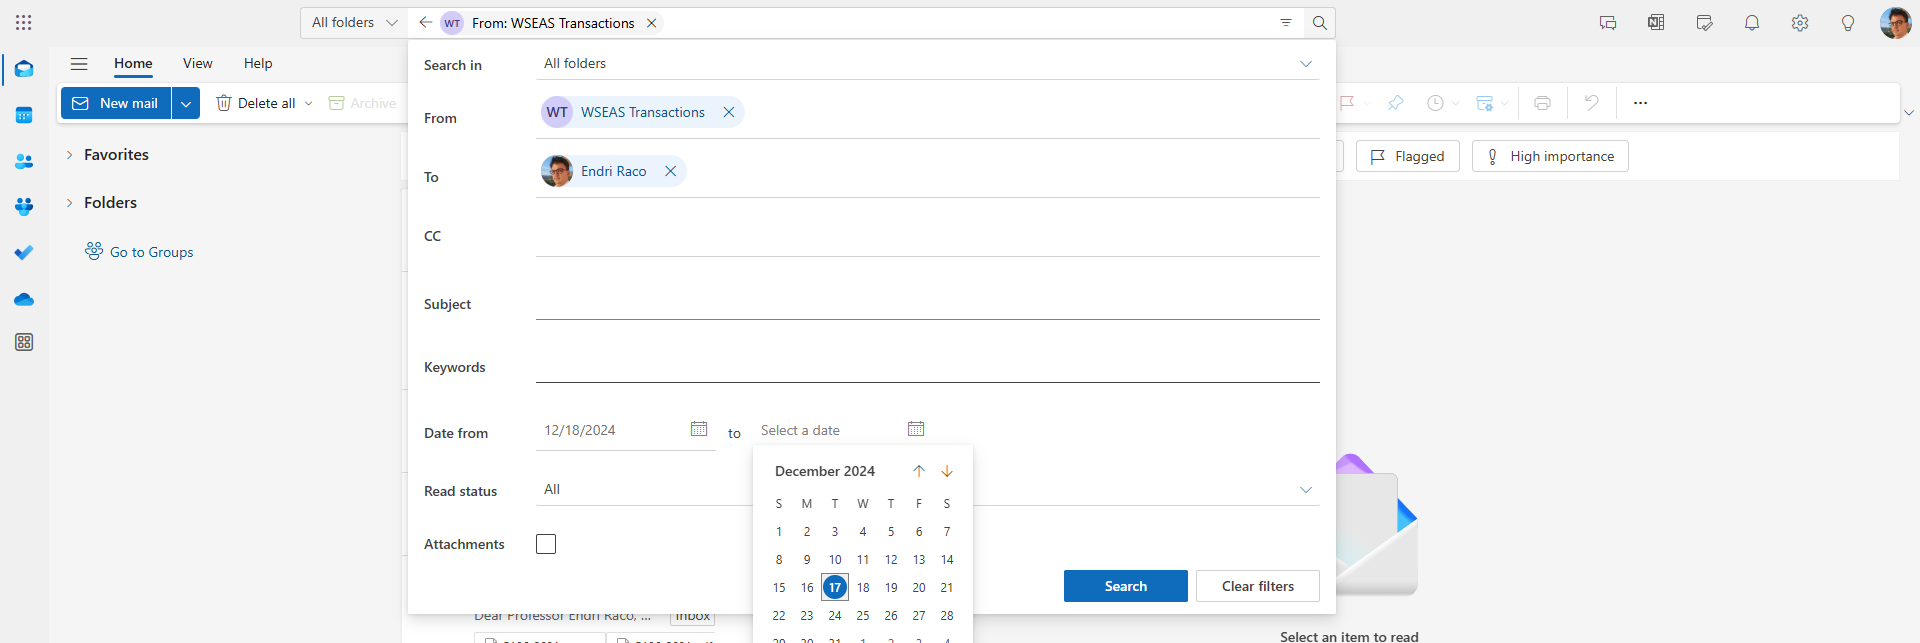
\includegraphics{./images/outlook20.png}
\end{frame}

\begin{frame}{Hapi 5: Kërkimi në dosje specifike}
\phantomsection\label{hapi-5-kuxebrkimi-nuxeb-dosje-specifike}
\begin{enumerate}
\item
  Nga shiriti i kërkimit, klikoni në \textbf{``Search in''}.
\item
  Zgjidhni një dosje specifike për të kërkuar:

  \begin{itemize}
  \item
    \textbf{Inbox} (Email-et e ardhura).
  \item
    \textbf{Sent Items} (Email-et e dërguara).
  \item
    \textbf{Deleted Items} (Email-et e fshira).
  \end{itemize}
\end{enumerate}
\end{frame}

\begin{frame}{Hapi 5: Kërkimi në dosje specifike}
\phantomsection\label{hapi-5-kuxebrkimi-nuxeb-dosje-specifike-1}
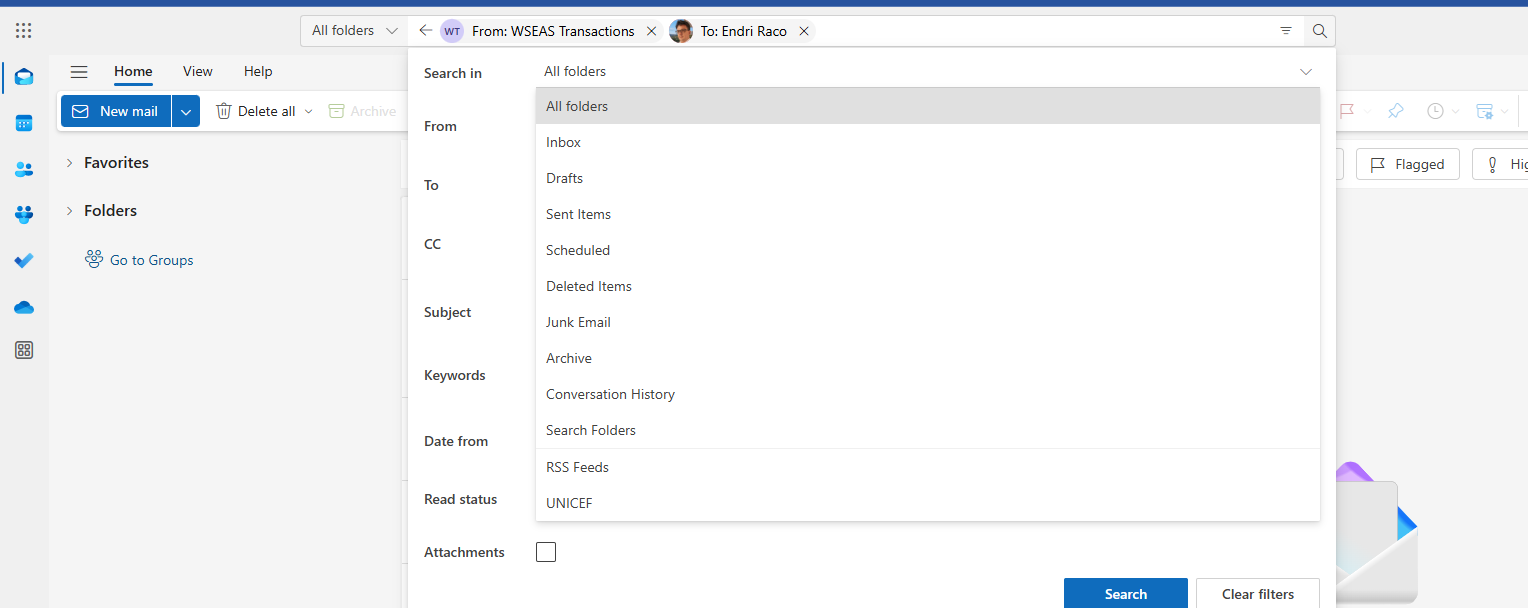
\includegraphics{./images/outlook21.png}
\end{frame}

\begin{frame}{Shembuj praktikë të kërkimit}
\phantomsection\label{shembuj-praktikuxeb-tuxeb-kuxebrkimit}
\begin{itemize}
\item
  \textbf{Kërkimi i emaileve nga një person specifik}:

  \begin{itemize}
  \tightlist
  \item
    \textbf{From: Endri Raço}
  \end{itemize}
\item
  \textbf{Kërkimi i emaileve me bashkëngjitje}:

  \begin{itemize}
  \tightlist
  \item
    \textbf{Has attachment: Yes}
  \end{itemize}
\item
  \textbf{Kërkimi i emaileve me një fjalë kyçe në subjekt}:

  \begin{itemize}
  \tightlist
  \item
    \textbf{Subject: raporti}
  \end{itemize}
\end{itemize}
\end{frame}

\begin{frame}{Përfitimet e përdorimit të kërkimit}
\phantomsection\label{puxebrfitimet-e-puxebrdorimit-tuxeb-kuxebrkimit}
\begin{itemize}
\item
  \textbf{Kursim kohe}: Gjeni emailet brenda sekondave.
\item
  \textbf{Organizim më i mirë}: Filtroni emailet sipas kritereve të
  rëndësishme.
\item
  \textbf{Qartësi dhe efikasitet}: Fokusohuni vetëm në emailet që ju
  nevojiten.
\end{itemize}
\end{frame}

\begin{frame}{Rezultate}
\phantomsection\label{rezultate}
\begin{itemize}
\item
  \textbf{Funksioni i kërkimit} në Outlook Web është një mjet i fuqishëm
  për të organizuar dhe gjetur emailet.
\item
  Praktikoni përdorimin e \textbf{filtrave} dhe \textbf{kërkimit të
  avancuar} për të rritur produktivitetin tuaj.
\end{itemize}
\end{frame}

\begin{frame}{Pyetje \& Diskutim}
\phantomsection\label{pyetje-diskutim-3}
\begin{itemize}
\tightlist
\item
  Cilat janë sfidat tuaja kryesore në kërkimin e emaileve?
\end{itemize}
\end{frame}

\begin{frame}{Menaxhimi i kontakteve}
\phantomsection\label{menaxhimi-i-kontakteve}
\begin{itemize}
\item
  Menaxhimi i kontakteve në \textbf{Outlook 365 Web} është një mënyrë
  efikase për të:

  \begin{itemize}
  \item
    Ruajtur informacionin e bashkëpunëtorëve dhe klientëve.
  \item
    Dërguar emaile më shpejt duke përdorur listat e kontakteve.
  \item
    Organizuar kontaktet në mënyrë të strukturuar.
  \end{itemize}
\end{itemize}
\end{frame}

\begin{frame}{Hapi 1: Hyrja në seksionin e kontakteve}
\phantomsection\label{hapi-1-hyrja-nuxeb-seksionin-e-kontakteve}
\begin{enumerate}
\item
  Klikoni ikonën e \textbf{``People''} (Njerëz) në këndin e poshtëm
  majtas.

  \begin{itemize}
  \tightlist
  \item
    Kjo do t'ju çojë te seksioni i kontakteve të Outlook Web.
  \end{itemize}
\end{enumerate}
\end{frame}

\begin{frame}{Hapi 1: Hyrja në seksionin e kontakteve}
\phantomsection\label{hapi-1-hyrja-nuxeb-seksionin-e-kontakteve-1}
\begin{enumerate}
\setcounter{enumi}{1}
\tightlist
\item
  Do të shihni listën tuaj të kontakteve ekzistuese.
\end{enumerate}

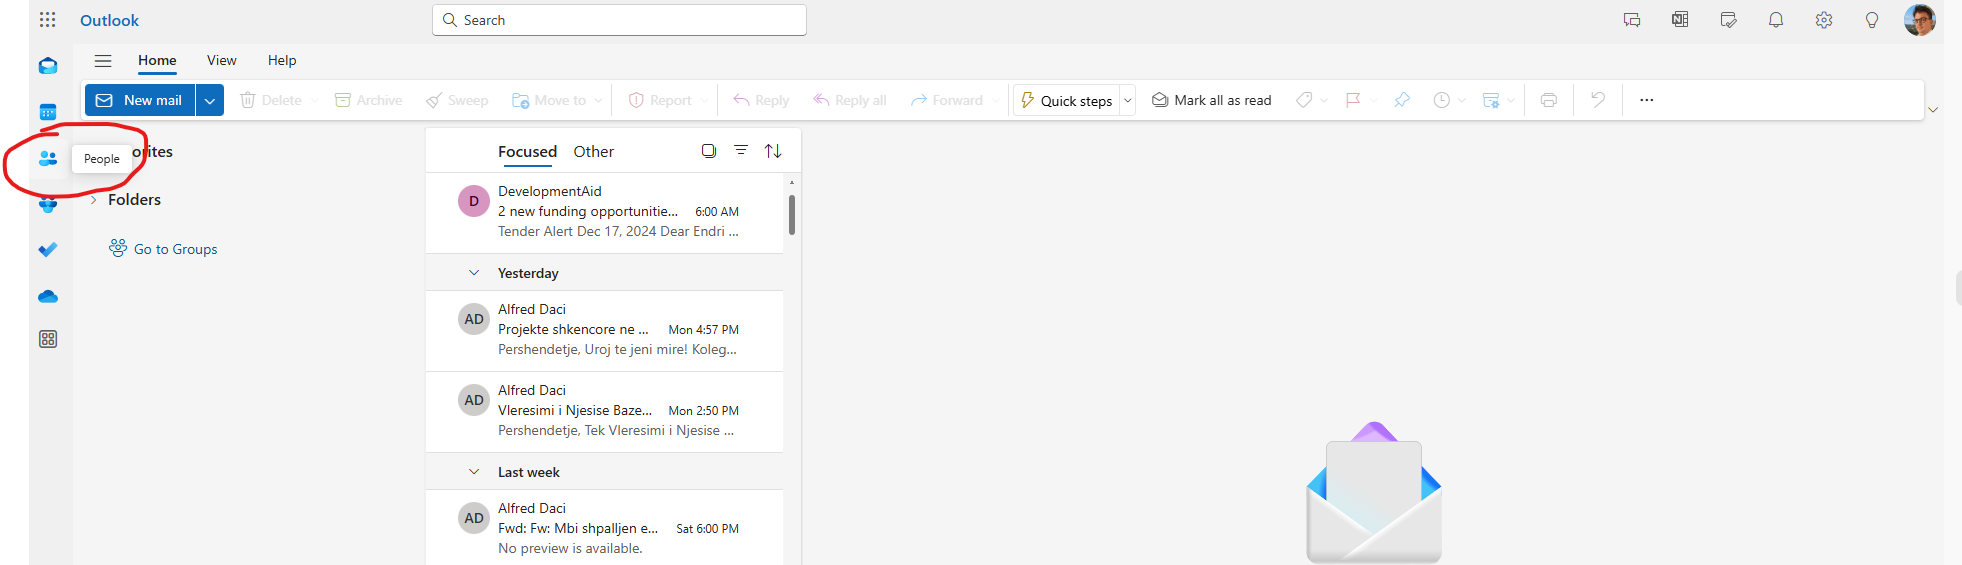
\includegraphics{./images/outlook22.png}
\end{frame}

\begin{frame}{Hapi 2: Shtimi i një kontakti të ri}
\phantomsection\label{hapi-2-shtimi-i-njuxeb-kontakti-tuxeb-ri}
\begin{enumerate}
\item
  Klikoni butonin \textbf{``New Contact''} (Kontakt i Ri).
\item
  Plotësoni fushat e nevojshme:

  \begin{itemize}
  \item
    \textbf{First Name} (Emri)
  \item
    \textbf{Last Name} (Mbiemri)
  \item
    \textbf{Email Address} (Adresa e email-it)
  \item
    \textbf{Phone Number} (Numri i telefonit) -- opsionale
  \end{itemize}
\end{enumerate}
\end{frame}

\begin{frame}{Hapi 2: Shtimi i një kontakti të ri}
\phantomsection\label{hapi-2-shtimi-i-njuxeb-kontakti-tuxeb-ri-1}
\begin{enumerate}
\setcounter{enumi}{2}
\tightlist
\item
  Klikoni \textbf{Save} (Ruaj) për ta shtuar kontaktin.
\end{enumerate}

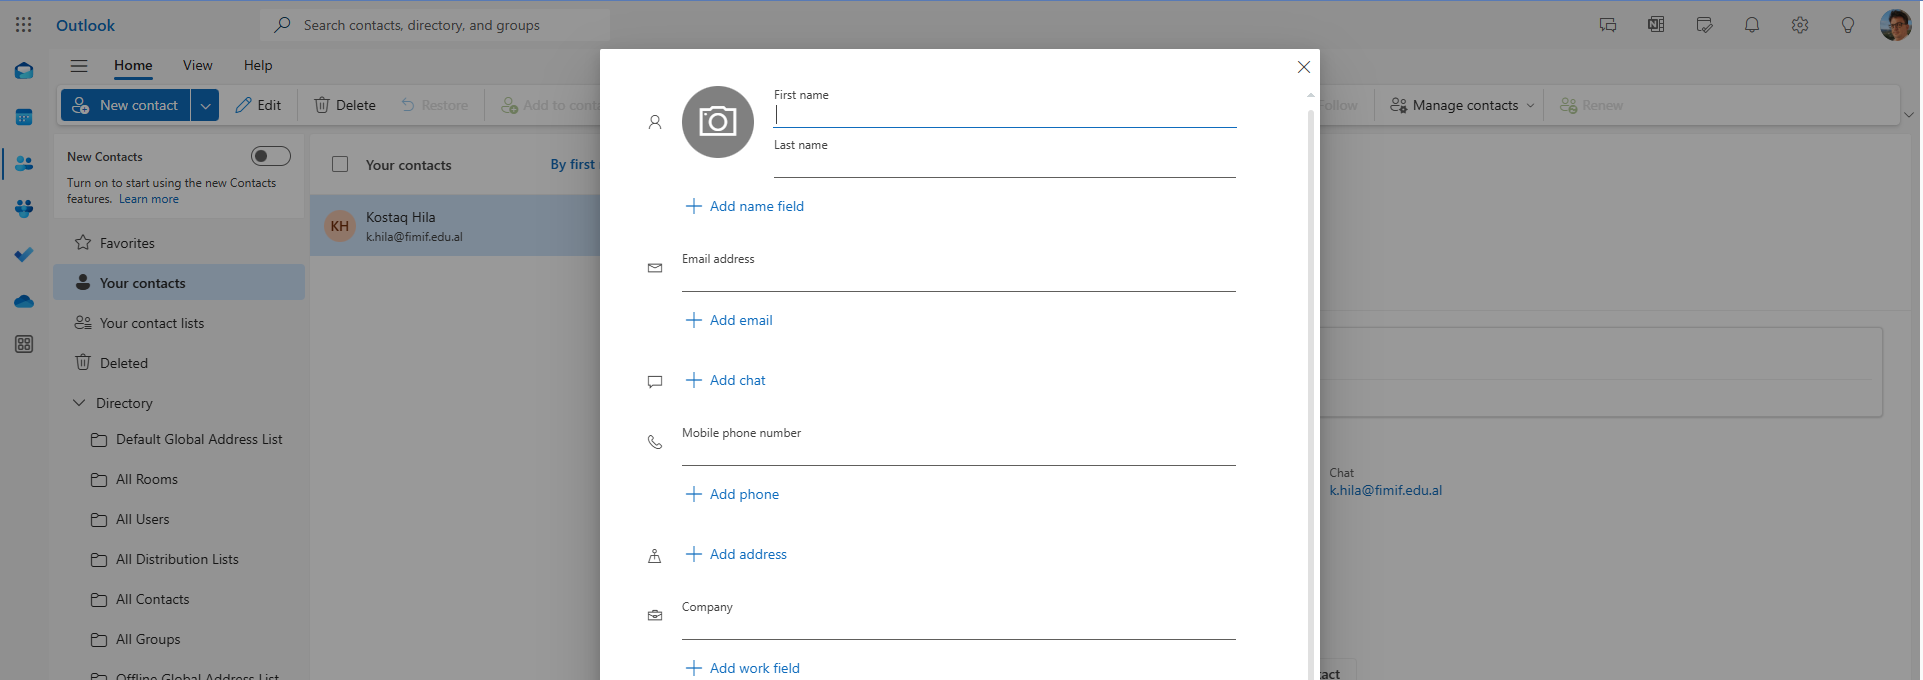
\includegraphics{./images/outlook23.png}
\end{frame}

\begin{frame}{Hapi 3: Krijimi i një grupi kontaktesh}
\phantomsection\label{hapi-3-krijimi-i-njuxeb-grupi-kontaktesh}
\begin{enumerate}
\item
  Klikoni \textbf{``New Contact List''} (Listë e Re Kontaktesh).
\item
  Vendosni një \textbf{emër} për listën, p.sh., \textbf{``Ekipi i
  Projektit''}.
\end{enumerate}
\end{frame}

\begin{frame}{Hapi 3: Krijimi i një grupi kontaktesh}
\phantomsection\label{hapi-3-krijimi-i-njuxeb-grupi-kontaktesh-1}
\begin{enumerate}
\setcounter{enumi}{2}
\item
  Shtoni kontaktet duke futur adresat e tyre të email-it.
\item
  Klikoni \textbf{Save} për të ruajtur listën.
\end{enumerate}

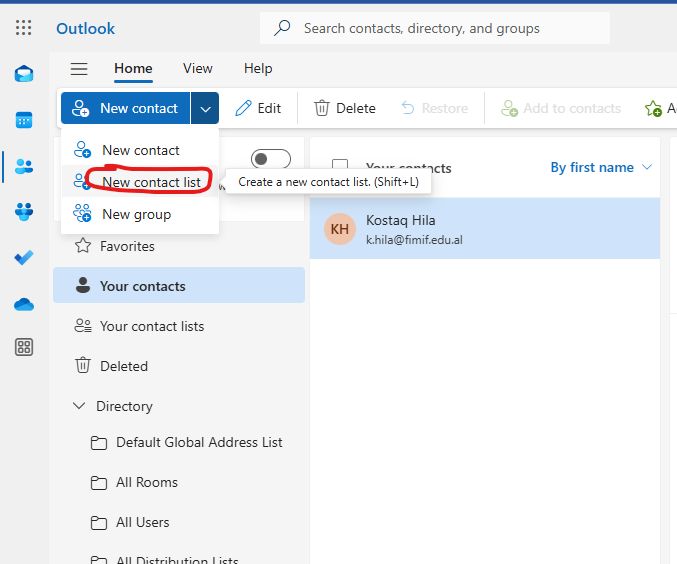
\includegraphics{./images/outlook24.png}
\end{frame}

\begin{frame}{Hapi 4: Redaktimi dhe fshirja e kontakteve}
\phantomsection\label{hapi-4-redaktimi-dhe-fshirja-e-kontakteve}
\begin{enumerate}
\item
  Për të \textbf{redaktuar} një kontakt:

  \begin{itemize}
  \item
    Klikoni mbi kontaktin dhe zgjidhni \textbf{``Edit''} (Redakto).
  \item
    Bëni ndryshimet dhe klikoni \textbf{Save} (Ruaj).
  \end{itemize}
\end{enumerate}
\end{frame}

\begin{frame}{Hapi 4: Redaktimi dhe fshirja e kontakteve}
\phantomsection\label{hapi-4-redaktimi-dhe-fshirja-e-kontakteve-1}
\begin{enumerate}
\setcounter{enumi}{1}
\item
  Për të \textbf{fshirë} një kontakt:

  \begin{itemize}
  \tightlist
  \item
    Klikoni mbi kontaktin dhe zgjidhni \textbf{``Delete''} (Fshi).
  \end{itemize}
\end{enumerate}

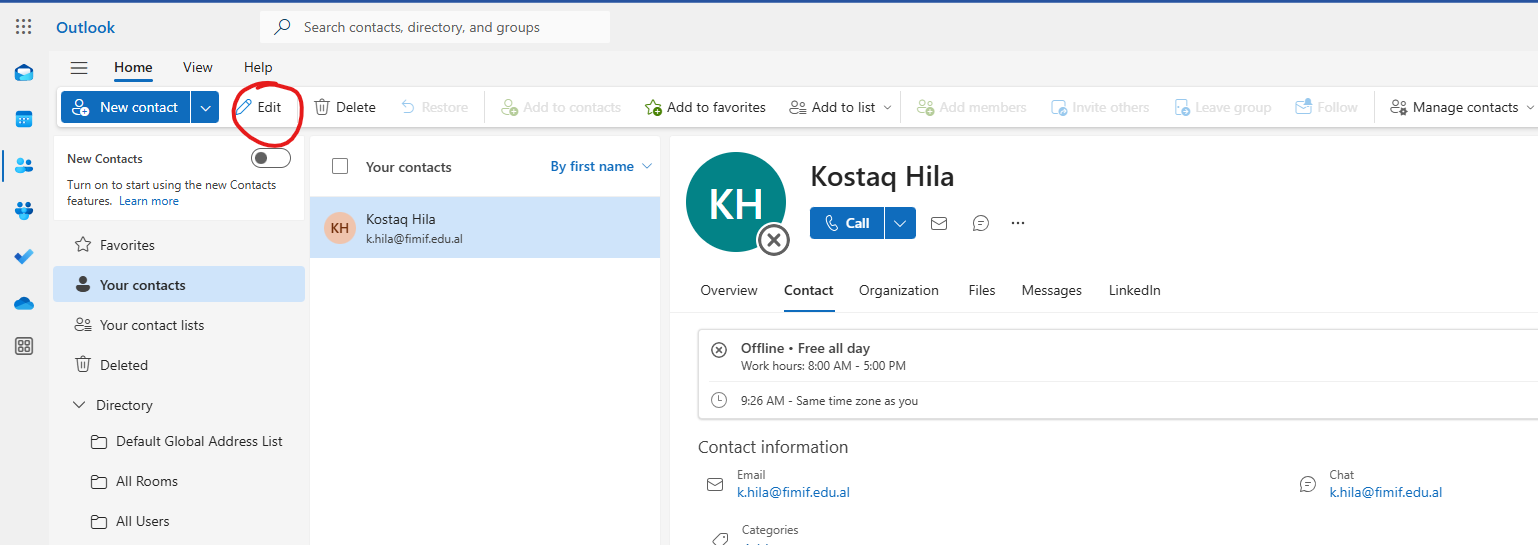
\includegraphics{./images/outlook25.png}
\end{frame}

\begin{frame}{Hapi 5: Kërkimi i kontakteve}
\phantomsection\label{hapi-5-kuxebrkimi-i-kontakteve}
\begin{enumerate}
\item
  Përdorni shiritin e kërkimit në seksionin \textbf{People}.
\item
  Shkruani emrin ose adresën e email-it të kontaktit që kërkoni.
\end{enumerate}
\end{frame}

\begin{frame}{Hapi 5: Kërkimi i kontakteve}
\phantomsection\label{hapi-5-kuxebrkimi-i-kontakteve-1}
\begin{enumerate}
\setcounter{enumi}{2}
\tightlist
\item
  Rezultatet do të shfaqen automatikisht.
\end{enumerate}

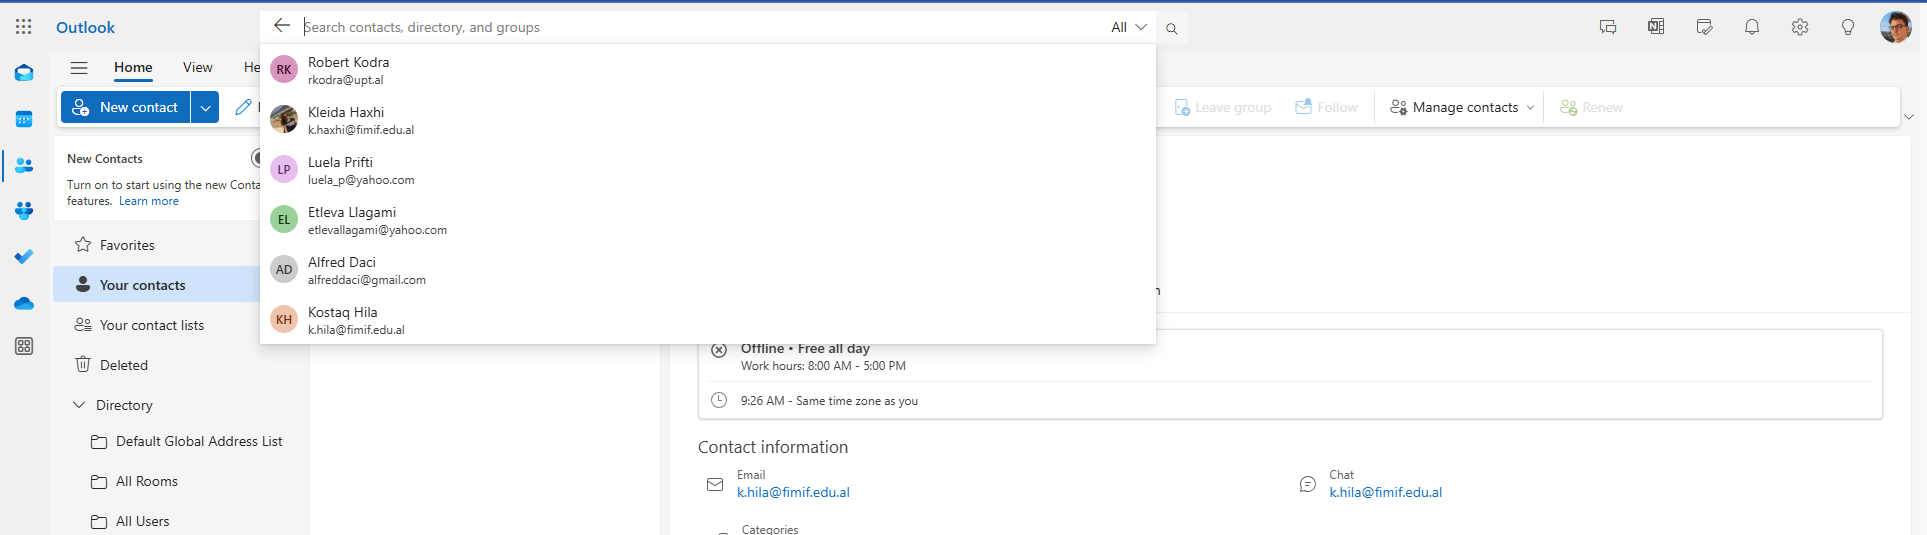
\includegraphics{./images/outlook26.png}
\end{frame}

\begin{frame}{Përfitimet e menaxhimit të kontakteve}
\phantomsection\label{puxebrfitimet-e-menaxhimit-tuxeb-kontakteve}
\begin{itemize}
\item
  \textbf{Organizim}: Të gjitha kontaktet ruhen në një vend të vetëm.
\item
  \textbf{Produktivitet}: Shkruani emaile më shpejt duke përdorur lista
  të kontakteve.
\item
  \textbf{Personalizim}: Mbani informacion të detajuar për secilin
  kontakt.
\end{itemize}
\end{frame}

\begin{frame}{Rezultate}
\phantomsection\label{rezultate-1}
\begin{itemize}
\item
  Menaxhimi i kontakteve në \textbf{Outlook 365 Web} është i lehtë dhe i
  shpejtë.
\item
  Përdorni funksionet për \textbf{krijimin}, \textbf{redaktimin} dhe
  \textbf{organizimin} e kontakteve për të përmirësuar komunikimin tuaj.
\end{itemize}
\end{frame}

\begin{frame}{Pyetje \& Diskutim}
\phantomsection\label{pyetje-diskutim-4}
\begin{itemize}
\tightlist
\item
  A keni përdorur më parë funksionin për menaxhimin e kontakteve?
\end{itemize}
\end{frame}

\begin{frame}{Funksioni i kalendarit}
\phantomsection\label{funksioni-i-kalendarit}
\begin{itemize}
\item
  \textbf{Funksioni i kalendarit} në Outlook 365 Web ju lejon të
  organizoni dhe ndani:

  \begin{itemize}
  \item
    Takime dhe ngjarje.
  \item
    Orarin tuaj me kolegët dhe bashkëpunëtorët.
  \end{itemize}
\item
  Ndaj kalendarin për të rritur \textbf{bashkëpunimin} dhe për të
  shmangur mbivendosjen e takimeve.
\end{itemize}
\end{frame}

\begin{frame}{Hapi 1: Hapja e Kalendarit}
\phantomsection\label{hapi-1-hapja-e-kalendarit}
\begin{enumerate}
\item
  Në panelin e majtë të Outlook, klikoni ikonën \textbf{``Calendar''}
  (Kalendar).

  \begin{itemize}
  \tightlist
  \item
    Kjo do të hapë pamjen e kalendarit tuaj.
  \end{itemize}
\end{enumerate}
\end{frame}

\begin{frame}{Hapi 1: Hapja e Kalendarit}
\phantomsection\label{hapi-1-hapja-e-kalendarit-1}
\begin{enumerate}
\setcounter{enumi}{1}
\tightlist
\item
  Kontrolloni opsionet si \textbf{Day}, \textbf{Week} dhe \textbf{Month}
  për pamje të ndryshme.
\end{enumerate}

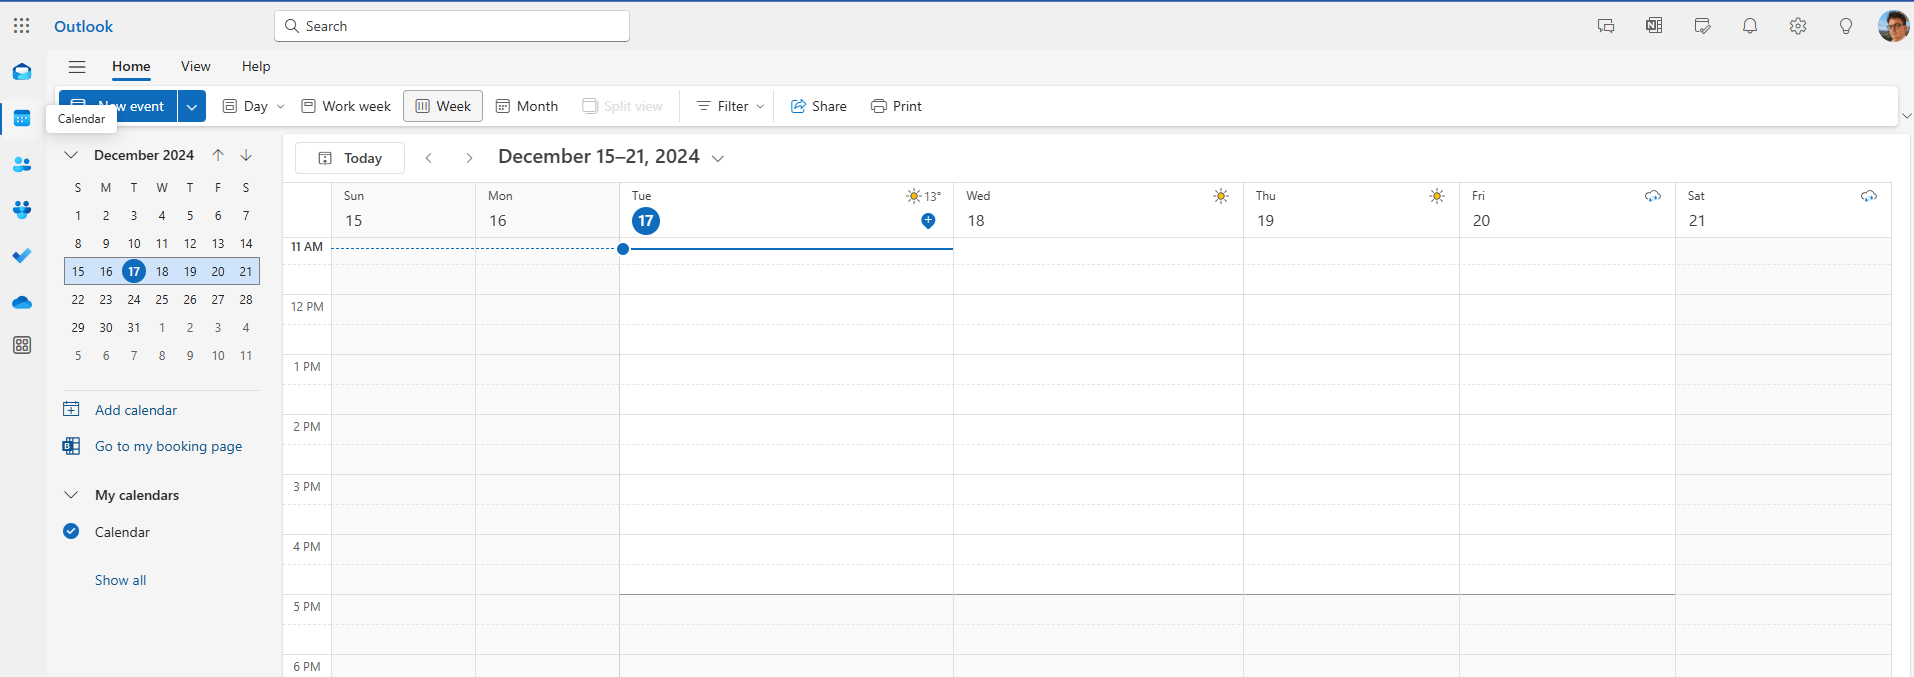
\includegraphics{./images/outlook27.png}
\end{frame}

\begin{frame}{Hapi 2: Ndani kalendarin tuaj}
\phantomsection\label{hapi-2-ndani-kalendarin-tuaj}
\begin{enumerate}
\tightlist
\item
  Klikoni mbi butonin \textbf{``Share''} (Ndaj) në këndin e sipërm
  djathtas.
\end{enumerate}

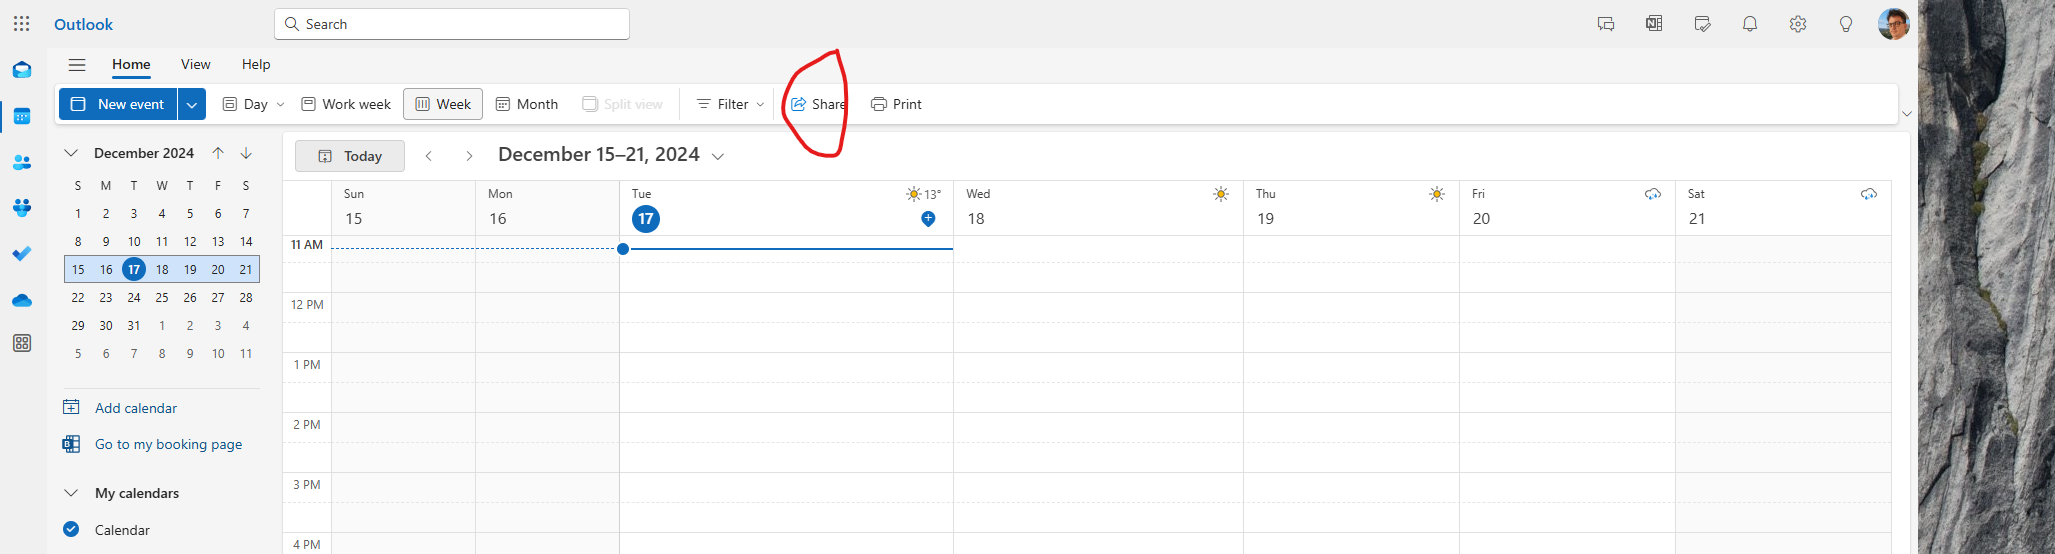
\includegraphics{./images/outlook28.png}
\end{frame}

\begin{frame}{Hapi 2: Ndani kalendarin tuaj}
\phantomsection\label{hapi-2-ndani-kalendarin-tuaj-1}
\begin{enumerate}
\setcounter{enumi}{1}
\tightlist
\item
  Në kutinë që shfaqet:

  \begin{itemize}
  \tightlist
  \item
    Futni adresën e email-it të personit me të cilin dëshironi ta ndani
    kalendarin.
  \end{itemize}
\end{enumerate}
\end{frame}

\begin{frame}{Hapi 2: Ndani kalendarin tuaj}
\phantomsection\label{hapi-2-ndani-kalendarin-tuaj-2}
\begin{itemize}
\item
  Zgjidhni nivelin e lejeve:

  \begin{itemize}
  \item
    \textbf{Can view when I'm busy} (Mund të shohë vetëm kur jeni të
    zënë).
  \item
    \textbf{Can view titles and locations} (Mund të shohë titujt dhe
    vendndodhjet).
  \item
    \textbf{Can view all details} (Mund të shohë të gjitha detajet).
  \item
    \textbf{Can edit} (Mund të redaktojë kalendarin tuaj).
  \end{itemize}
\end{itemize}
\end{frame}

\begin{frame}{Hapi 2: Ndani kalendarin tuaj}
\phantomsection\label{hapi-2-ndani-kalendarin-tuaj-3}
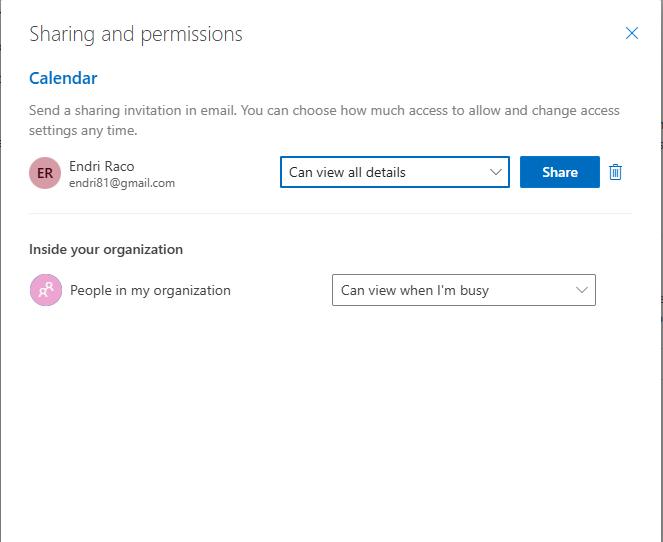
\includegraphics{./images/outlook29.png}
\end{frame}

\begin{frame}{Hapi 3: Dërgimi i ftesës për ndarjen}
\phantomsection\label{hapi-3-duxebrgimi-i-ftesuxebs-puxebr-ndarjen}
\begin{enumerate}
\item
  Klikoni \textbf{``Share''} për të dërguar ftesën.
\item
  Marrësi do të marrë një email për të pranuar ftesën.
\end{enumerate}
\end{frame}

\begin{frame}{Hapi 4: Kontrolli i lejeve të shpërndarjes}
\phantomsection\label{hapi-4-kontrolli-i-lejeve-tuxeb-shpuxebrndarjes}
\begin{enumerate}
\item
  Për të parë ose modifikuar se me kë e keni ndarë kalendarin:

  \begin{itemize}
  \tightlist
  \item
    Klikoni mbi \textbf{``Manage Permissions''} (Menaxho Lejet).
  \end{itemize}
\end{enumerate}

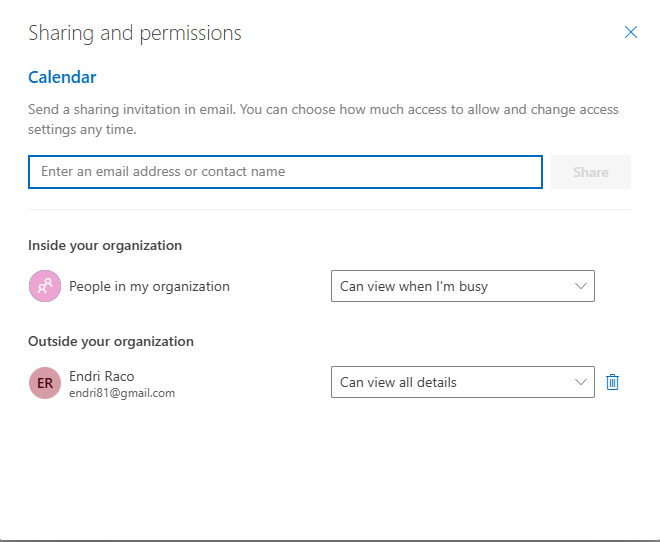
\includegraphics{./images/outlook30.png}
\end{frame}

\begin{frame}{Hapi 4: Kontrolli i lejeve të shpërndarjes}
\phantomsection\label{hapi-4-kontrolli-i-lejeve-tuxeb-shpuxebrndarjes-1}
\begin{enumerate}
\setcounter{enumi}{1}
\item
  Mund të:

  \begin{itemize}
  \item
    \textbf{Modifikoni lejet} për personat ekzistues.
  \item
    \textbf{Hiqni aksesin} për përdorues të veçantë.
  \end{itemize}
\end{enumerate}
\end{frame}

\begin{frame}{Shembull praktik}
\phantomsection\label{shembull-praktik}
\begin{itemize}
\item
  \textbf{Shembull}: Ndarja e kalendarit me ekipin për të planifikuar
  një mbledhje javore:

  \begin{enumerate}
  \item
    Ndarja e kalendarit me \textbf{Can view all details}.
  \item
    Caktimi i mbledhjeve duke përdorur pamjen \textbf{Week}.
  \end{enumerate}
\end{itemize}
\end{frame}

\begin{frame}{Përfitimet e ndarjes së kalendarit}
\phantomsection\label{puxebrfitimet-e-ndarjes-suxeb-kalendarit}
\begin{itemize}
\item
  \textbf{Transparencë}: Të tjerët mund të shohin disponueshmërinë tuaj.
\item
  \textbf{Efikasitet}: Planifikimi i takimeve bëhet më i lehtë.
\item
  \textbf{Bashkëpunim}: Koordinim më i mirë në projekte dhe aktivitete.
\end{itemize}
\end{frame}

\begin{frame}{Rezultate}
\phantomsection\label{rezultate-2}
\begin{itemize}
\item
  Ndarja e kalendarit tuaj në Outlook 365 Web është një mënyrë e
  thjeshtë për të rritur \textbf{bashkëpunimin} dhe
  \textbf{organizimin}.
\item
  Përdorni funksionet për \textbf{menaxhimin e lejeve} për të
  kontrolluar aksesin.
\end{itemize}
\end{frame}

\begin{frame}{Pyetje \& Diskutim}
\phantomsection\label{pyetje-diskutim-5}
\begin{itemize}
\tightlist
\item
  A keni ndarë ndonjëherë kalendarin tuaj me kolegët?
\end{itemize}
\end{frame}

\begin{frame}{Programimi i emaileve}
\phantomsection\label{programimi-i-emaileve}
\begin{itemize}
\item
  \textbf{Programimi i emaileve} ju lejon të dërgoni mesazhe në një kohë
  të caktuar në të ardhmen.
\item
  Kjo është e dobishme për:

  \begin{itemize}
  \item
    Dërgimin e emaileve në orare të përshtatshme për marrësit.
  \item
    Kujtesa të planifikuara për projekte dhe takime.
  \item
    Rritjen e produktivitetit dhe organizimit.
  \end{itemize}
\end{itemize}
\end{frame}

\begin{frame}{Hapi 1: Krijimi i një email-i të ri}
\phantomsection\label{hapi-1-krijimi-i-njuxeb-email-i-tuxeb-ri}
\begin{enumerate}
\item
  Klikoni mbi butonin \textbf{``New Email''} (Email i Ri) në këndin e
  sipërm majtas.
\item
  Plotësoni detajet e email-it:

  \begin{itemize}
  \item
    \textbf{To}: Adresa e marrësit.
  \item
    \textbf{Subject}: Subjekti i email-it.
  \item
    \textbf{Body}: Përmbajtja e mesazhit.
  \end{itemize}
\end{enumerate}
\end{frame}

\begin{frame}{Hapi 1: Krijimi i një email-i të ri}
\phantomsection\label{hapi-1-krijimi-i-njuxeb-email-i-tuxeb-ri-1}
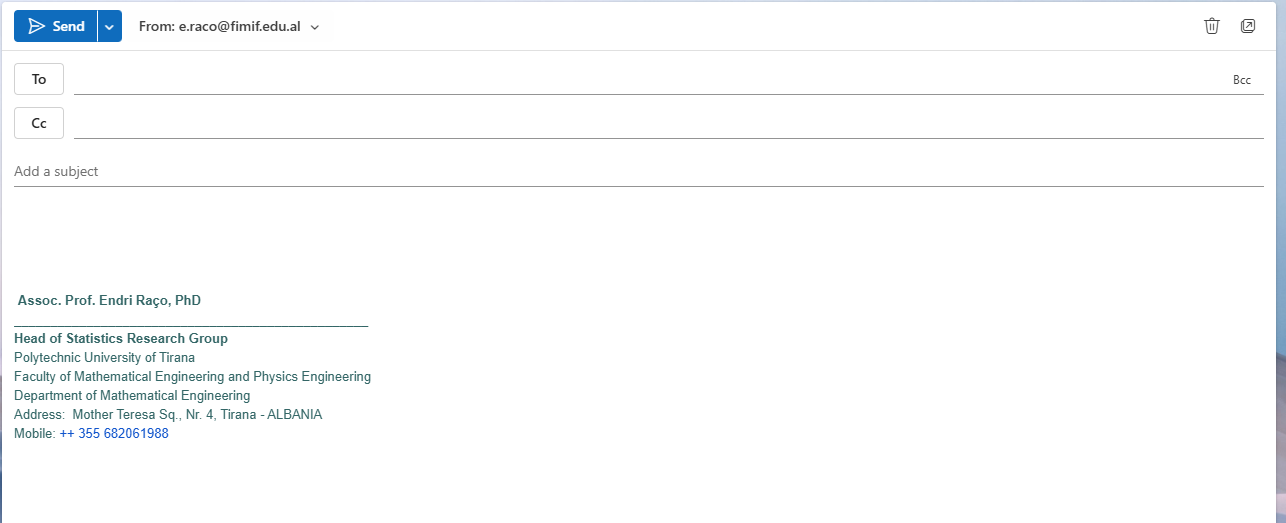
\includegraphics{./images/outlook31.png}
\end{frame}

\begin{frame}{Hapi 2: Programimi i dërgimit të email-it}
\phantomsection\label{hapi-2-programimi-i-duxebrgimit-tuxeb-email-it}
\begin{enumerate}
\item
  Klikoni mbi shigjetën poshtë \textbf{butonit Send} (Dërgo).
\item
  Zgjidhni opsionin \textbf{``Schedule Send''} (Programo Dërgimin).
\end{enumerate}

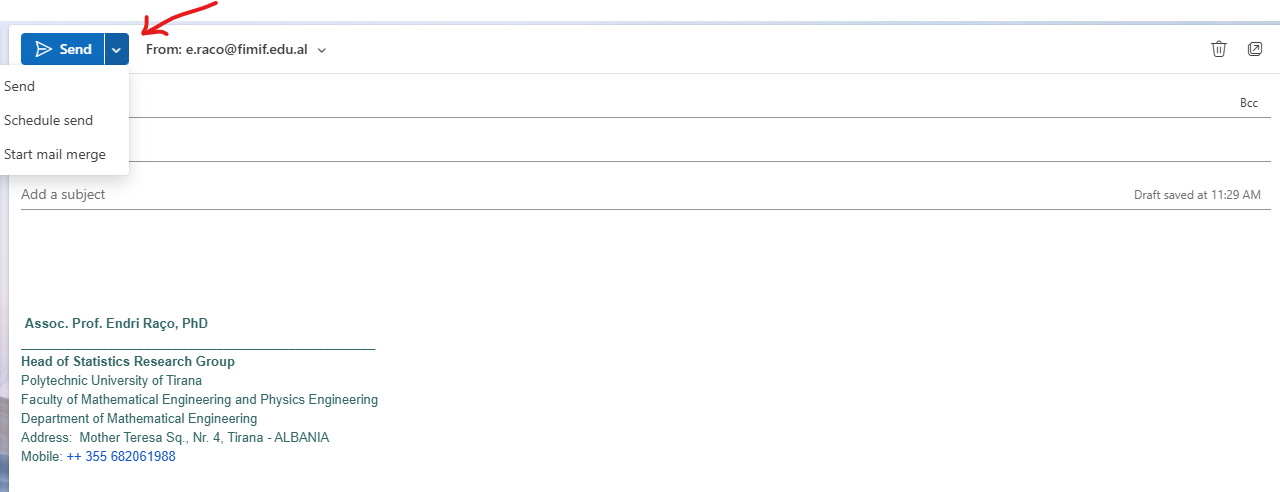
\includegraphics{./images/outlook32.png}
\end{frame}

\begin{frame}{Hapi 3: Zgjedhja e datës dhe kohës}
\phantomsection\label{hapi-3-zgjedhja-e-datuxebs-dhe-kohuxebs}
\begin{enumerate}
\item
  Një dritare do të shfaqet për të vendosur \textbf{datën dhe orën} e
  dërgimit.
\item
  Zgjidhni datën dhe kohën e dëshiruar.
\end{enumerate}

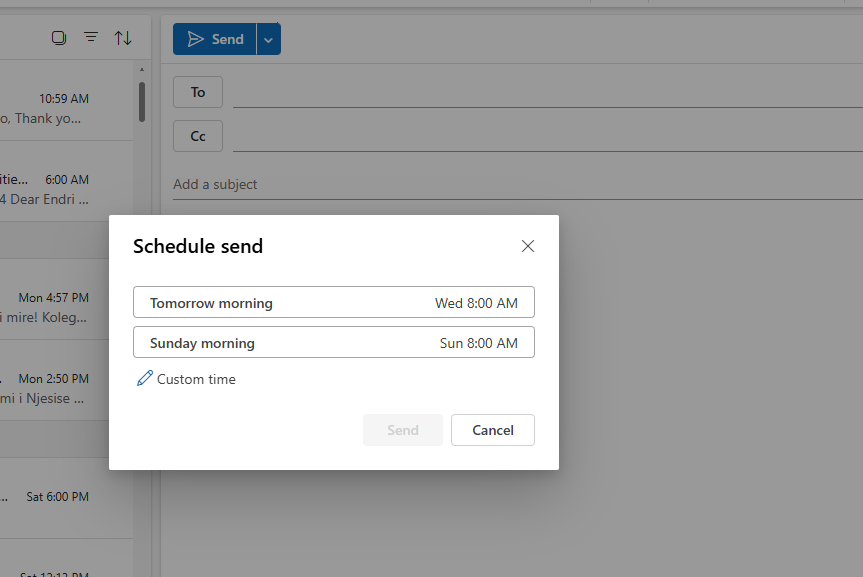
\includegraphics{./images/outlook33.png}
\end{frame}

\begin{frame}{Hapi 3: Zgjedhja e datës dhe kohës}
\phantomsection\label{hapi-3-zgjedhja-e-datuxebs-dhe-kohuxebs-1}
\begin{enumerate}
\setcounter{enumi}{2}
\tightlist
\item
  Klikoni \textbf{``Send''} për të programuar email-in.
\end{enumerate}
\end{frame}

\begin{frame}{Hapi 5: Kontrolli i emaileve të programuar}
\phantomsection\label{hapi-5-kontrolli-i-emaileve-tuxeb-programuar}
\begin{enumerate}
\item
  Për të parë emailet e programuar:

  \begin{itemize}
  \tightlist
  \item
    Shkoni te \textbf{``Drafts''} ose te \textbf{``Scheduled''} në
    panelin e majtë.
  \end{itemize}
\item
  Klikoni mbi email-in për ta modifikuar ose për të ndryshuar orarin e
  dërgimit.
\end{enumerate}
\end{frame}

\begin{frame}{Shembull praktik}
\phantomsection\label{shembull-praktik-1}
\begin{itemize}
\item
  \textbf{Shembull}: Programoni një email që do të dërgohet nesër në
  orën 9:00 për të njoftuar ekipin tuaj për një mbledhje:

  \begin{itemize}
  \item
    Adresa:
    \textbf{\href{mailto:ekipi@shembull.com}{\nolinkurl{ekipi@shembull.com}}}
  \item
    Subjekti: \textbf{Njoftim për mbledhjen e nesërme}.
  \item
    Koha: \textbf{9:00 AM}.
  \end{itemize}
\end{itemize}
\end{frame}

\begin{frame}{Përfitimet e programimit të emaileve}
\phantomsection\label{puxebrfitimet-e-programimit-tuxeb-emaileve}
\begin{itemize}
\item
  \textbf{Planifikim më i mirë}: Organizoni dërgimin e mesazheve në
  orarin optimal.
\item
  \textbf{Kursim kohe}: Përgatitni emailet paraprakisht dhe programoni
  dërgimin.
\item
  \textbf{Profesionalizëm}: Dërgoni emaile në orare të përshtatshme për
  marrësit.
\end{itemize}
\end{frame}

\begin{frame}{Rezultate}
\phantomsection\label{rezultate-3}
\begin{itemize}
\item
  Funksioni \textbf{``Schedule Send''} në Outlook 365 Web është një
  mënyrë efikase për të menaxhuar komunikimin tuaj me email.
\item
  Përdoreni këtë veçori për të rritur produktivitetin dhe për të
  planifikuar mesazhet sipas nevojës.
\end{itemize}
\end{frame}

\begin{frame}{Pyetje \& Diskutim}
\phantomsection\label{pyetje-diskutim-6}
\begin{itemize}
\tightlist
\item
  A e keni përdorur më parë funksionin \textbf{Schedule Send}?
\end{itemize}
\end{frame}

\begin{frame}{Përgjigjet automatike}
\phantomsection\label{puxebrgjigjet-automatike}
\begin{itemize}
\item
  \textbf{Përgjigjet automatike} ju lejojnë të njoftoni të tjerët kur
  nuk jeni të disponueshëm për të lexuar ose përgjigjur email-eve.
\item
  Kjo është e dobishme kur jeni në:

  \begin{itemize}
  \item
    Pushime.
  \item
    Takime ose ngjarje të zgjatura.
  \item
    Jashtë zyrës për periudha të caktuara.
  \end{itemize}
\end{itemize}
\end{frame}

\begin{frame}{Hapi 1: Hyrja në cilësimet e përgjigjeve automatike}
\phantomsection\label{hapi-1-hyrja-nuxeb-ciluxebsimet-e-puxebrgjigjeve-automatike}
\begin{enumerate}
\item
  Klikoni mbi ikonën e \textbf{``Settings''} në këndin e sipërm
  djathtas.
\item
  Klikoni mbi \textbf{``Accounts''} dhe \textbf{Automatic Replies}
\end{enumerate}

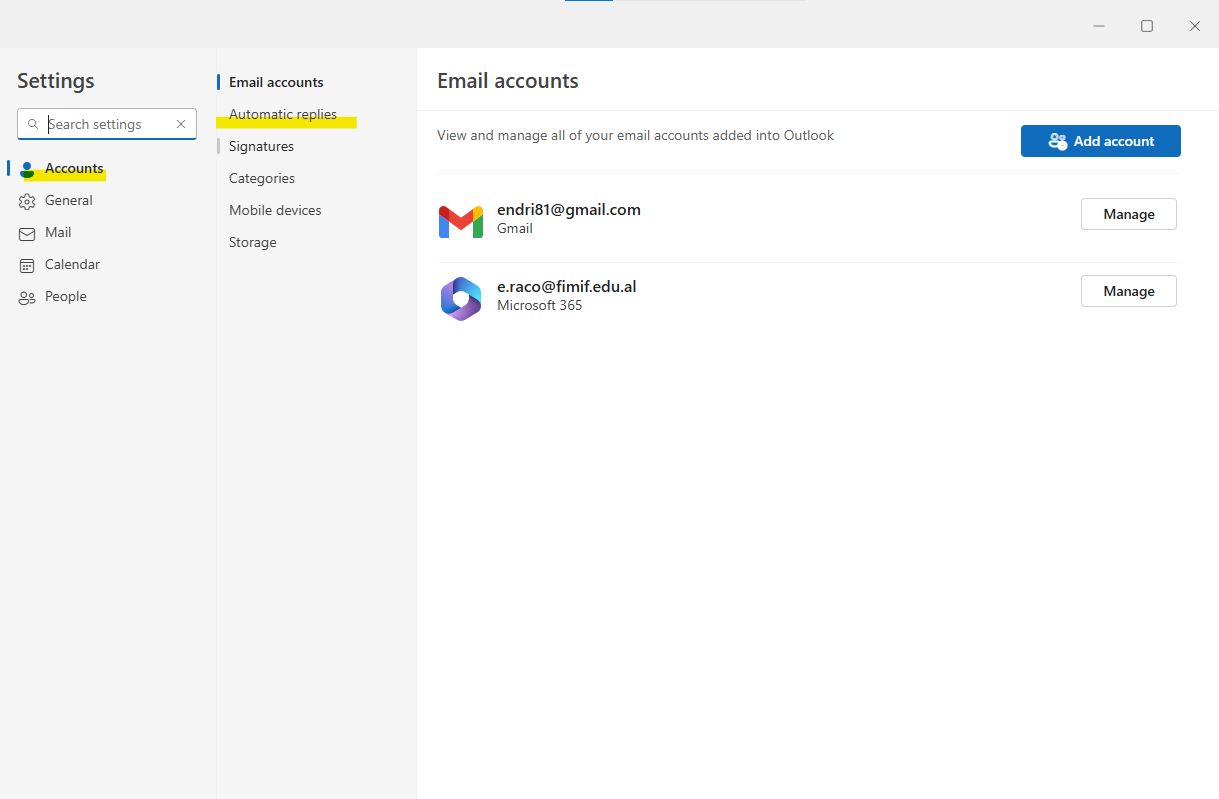
\includegraphics{./images/outlook34.png}
\end{frame}

\begin{frame}{Hapi 2: Aktivizimi i përgjigjeve automatike}
\phantomsection\label{hapi-2-aktivizimi-i-puxebrgjigjeve-automatike}
Aktivizoni opsionin \textbf{``Turn on automatic replies''} (Aktivizo
përgjigjet automatike).

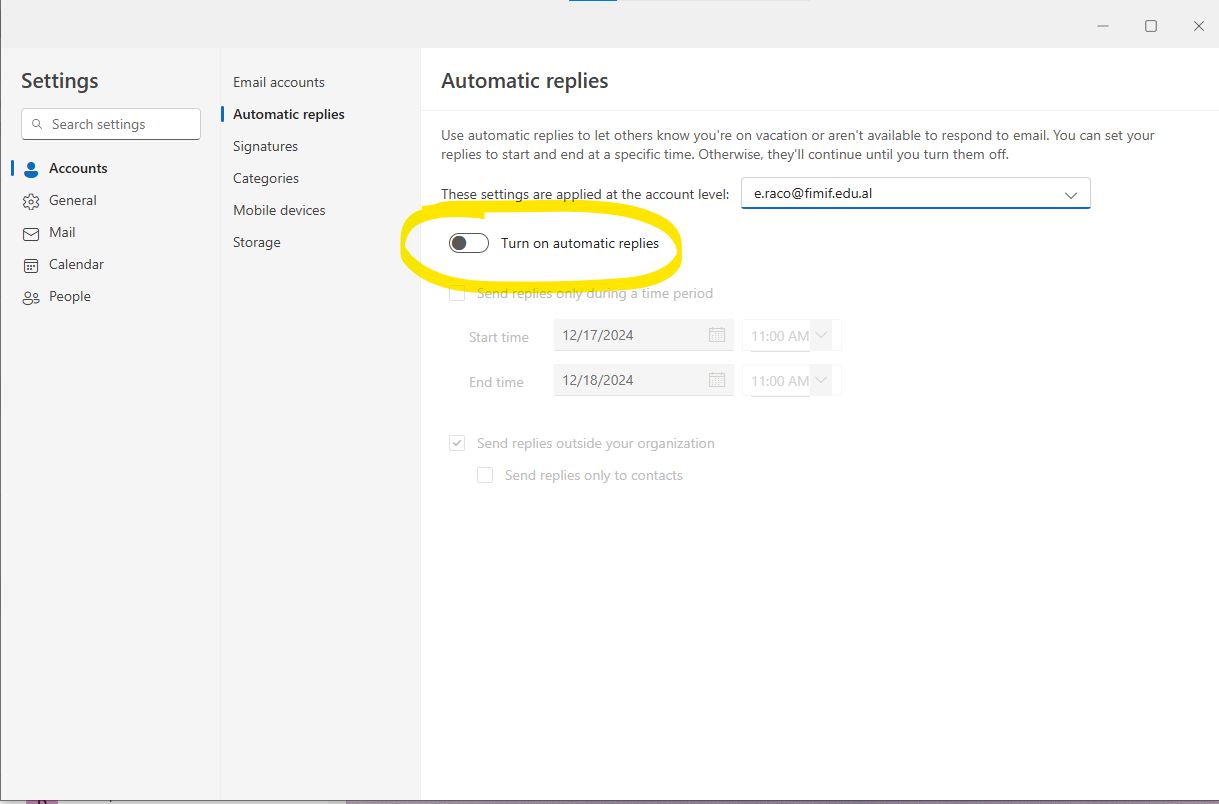
\includegraphics{./images/outlook35.png}
\end{frame}

\begin{frame}{Hapi 4: Vendosja e mesazhit automatik}
\phantomsection\label{hapi-4-vendosja-e-mesazhit-automatik}
\begin{enumerate}
\item
  Shkruani mesazhin që dëshironi t'u dërgohet të tjerëve:

  \begin{itemize}
  \tightlist
  \item
    P.sh.: \textbf{``Përshëndetje, jam me pushime deri më 15 Nëntor. Do
    t'ju përgjigjem sapo të kthehem. Faleminderit!''}
  \end{itemize}
\item
  Opsionale:

  \begin{itemize}
  \item
    Vendosni \textbf{datën dhe orën} kur përgjigjet automatike duhet të
    aktivizohen dhe të përfundojnë.
  \item
    Aktivizoni opsionin për të dërguar përgjigje vetëm për kontaktet
    tuaja të organizatës.
  \end{itemize}
\end{enumerate}
\end{frame}

\begin{frame}{Hapi 5: Ruajtja e cilësimeve}
\phantomsection\label{hapi-5-ruajtja-e-ciluxebsimeve}
\begin{enumerate}
\item
  Pasi të keni përfunduar mesazhin dhe opsionet, klikoni
  \textbf{``Save''} (Ruaj).
\item
  Një shenjë që përgjigjet automatike janë aktive do të shfaqet në krye
  të ekranit të Outlook.
\end{enumerate}
\end{frame}

\begin{frame}{Shembull praktik}
\phantomsection\label{shembull-praktik-2}
\begin{itemize}
\item
  \textbf{Shembull mesazhi për pushime}:

  ``Përshëndetje,\\
  Faleminderit për email-in tuaj. Jam me pushime deri më 20 Nëntor dhe
  nuk do të kem akses në email. Për çështje urgjente, ju lutem
  kontaktoni kolegun tim në:
  \href{mailto:kolegu@example.com}{\nolinkurl{kolegu@example.com}}.\\
  Faleminderit për mirëkuptimin!''
\end{itemize}
\end{frame}

\begin{frame}{Si të çaktivizoni përgjigjet automatike}
\phantomsection\label{si-tuxeb-uxe7aktivizoni-puxebrgjigjet-automatike}
\begin{enumerate}
\item
  Shkoni te \textbf{Settings \textgreater{} Accounts \textgreater{}
  Automatic replies}.
\item
  Çaktivizoni opsionin \textbf{``Turn off automatic replies''}
  (Çaktivizo përgjigjet automatike).
\item
  Klikoni \textbf{Save}.
\end{enumerate}
\end{frame}

\begin{frame}{Përfitimet e përdorimit të përgjigjeve automatike}
\phantomsection\label{puxebrfitimet-e-puxebrdorimit-tuxeb-puxebrgjigjeve-automatike}
\begin{itemize}
\item
  \textbf{Njoftoni të tjerët} për mungesën tuaj.
\item
  \textbf{Mbani profesionalizëm} në komunikim.
\item
  \textbf{Reduktoni pritshmëritë} për një përgjigje të shpejtë.
\end{itemize}
\end{frame}

\begin{frame}{Rezultate}
\phantomsection\label{rezultate-4}
\begin{itemize}
\item
  \textbf{Përgjigjet automatike} janë të lehta për t'u vendosur dhe ju
  ndihmojnë të menaxhoni komunikimin kur nuk jeni të disponueshëm.
\item
  Përdorni këtë funksion për të kursyer kohë dhe për të informuar
  kontaktet tuaja në mënyrë profesionale.
\end{itemize}
\end{frame}

\begin{frame}{Pyetje \& Diskutim}
\phantomsection\label{pyetje-diskutim-7}
\begin{itemize}
\tightlist
\item
  Keni hasur ndonjë vështirësi në vendosjen e përgjigjeve automatike?
\end{itemize}
\end{frame}

\section{Teams 365 Web}\label{teams-365-web}

\begin{frame}{Çfarë është Microsoft Teams?}
\phantomsection\label{uxe7faruxeb-uxebshtuxeb-microsoft-teams}
\begin{itemize}
\item
  \textbf{Microsoft Teams} është një platformë bashkëpunimi dhe
  komunikimi brenda \textbf{Office 365}.
\item
  Është krijuar për të ndihmuar ekipet të:

  \begin{itemize}
  \item
    \textbf{Komunikojnë} në kohë reale.
  \item
    \textbf{Bashkëpunojnë} në dokumente dhe projekte.
  \item
    Organizojnë \textbf{takime virtuale} dhe ndajnë informacione.
  \end{itemize}
\end{itemize}
\end{frame}

\begin{frame}{Çfarë është Microsoft Teams?}
\phantomsection\label{uxe7faruxeb-uxebshtuxeb-microsoft-teams-1}
\textbf{Microsoft Teams} bashkon funksionet e:

\begin{itemize}
\item
  \textbf{Chat} (Bisedë)
\item
  \textbf{Meetings} (Takime)
\item
  \textbf{Calls} (Thirrje)
\item
  \textbf{Files} (Skedarë dhe dokumente).
\end{itemize}
\end{frame}

\begin{frame}{Benefitet e përdorimit të Teams}
\phantomsection\label{benefitet-e-puxebrdorimit-tuxeb-teams}
\begin{enumerate}
\item
  \textbf{Komunikim i lehtë dhe i shpejtë}

  \begin{itemize}
  \item
    Bisedoni me ekipin tuaj në kohë reale.
  \item
    Biseda të organizuara sipas kanaleve dhe temave.
  \end{itemize}
\end{enumerate}
\end{frame}

\begin{frame}{Benefitet e përdorimit të Teams}
\phantomsection\label{benefitet-e-puxebrdorimit-tuxeb-teams-1}
\begin{enumerate}
\setcounter{enumi}{1}
\item
  \textbf{Bashkëpunim në dokumente}

  \begin{itemize}
  \tightlist
  \item
    Redaktoni dokumente në të njëjtën kohë me kolegët përmes
    \textbf{Word}, \textbf{Excel} dhe \textbf{PowerPoint}.
  \end{itemize}
\end{enumerate}
\end{frame}

\begin{frame}{Benefitet e përdorimit të Teams}
\phantomsection\label{benefitet-e-puxebrdorimit-tuxeb-teams-2}
\begin{enumerate}
\setcounter{enumi}{2}
\item
  \textbf{Takime virtuale}

  \begin{itemize}
  \item
    Organizoni \textbf{video takime} me një klikim.
  \item
    Ndani ekranin dhe prezantoni ide në mënyrë të qartë.
  \end{itemize}
\end{enumerate}
\end{frame}

\begin{frame}{Benefitet e përdorimit të Teams}
\phantomsection\label{benefitet-e-puxebrdorimit-tuxeb-teams-3}
\begin{enumerate}
\setcounter{enumi}{3}
\item
  \textbf{Fleksibilitet dhe akses}

  \begin{itemize}
  \tightlist
  \item
    Përdorimi i Microsoft Teams nga \textbf{çdo pajisje} dhe \textbf{çdo
    vend}.
  \end{itemize}
\end{enumerate}
\end{frame}

\begin{frame}{Si të filloni punën me Microsoft Teams?}
\phantomsection\label{si-tuxeb-filloni-punuxebn-me-microsoft-teams}
Hyrja në Microsoft Teams

\begin{enumerate}
\tightlist
\item
  Hapni shfletuesin dhe shkoni në:\\
  \textbf{\url{https://teams.microsoft.com}}
\end{enumerate}
\end{frame}

\begin{frame}{Si të filloni punën me Microsoft Teams?}
\phantomsection\label{si-tuxeb-filloni-punuxebn-me-microsoft-teams-1}
\begin{enumerate}
\setcounter{enumi}{1}
\tightlist
\item
  Identifikohuni me kredencialet tuaja të \textbf{Office 365}.
\end{enumerate}

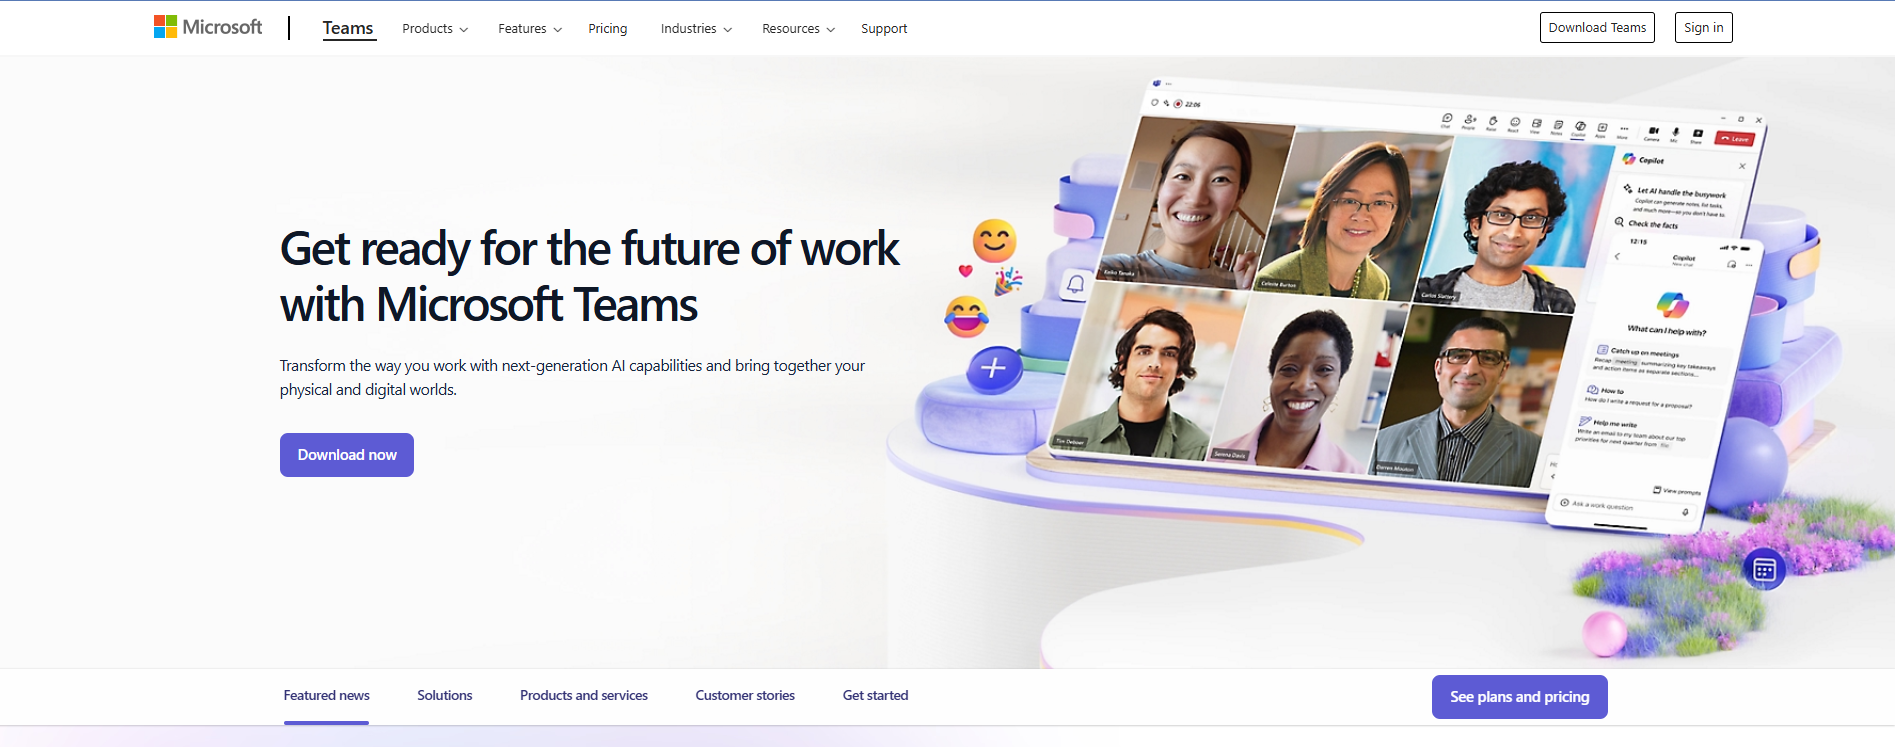
\includegraphics{./images/teams1.png}
\end{frame}

\begin{frame}{Navigimi në Teams}
\phantomsection\label{navigimi-nuxeb-teams}
\begin{itemize}
\item
  \textbf{Teams}: Hapësirat e organizuara për komunikim sipas projekteve
  ose departamenteve.
\item
  \textbf{Chat}: Biseda private ose në grup me kolegët.
\end{itemize}

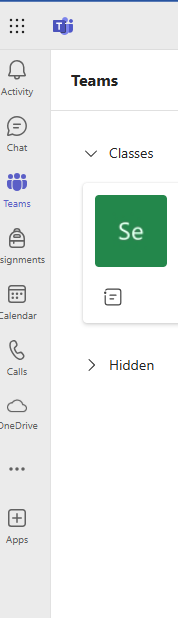
\includegraphics{./images/teams2.png}
\end{frame}

\begin{frame}{Navigimi në Teams}
\phantomsection\label{navigimi-nuxeb-teams-1}
\begin{itemize}
\item
  \textbf{Calendar}: Organizoni dhe planifikoni takime virtuale.
\item
  \textbf{Files}: Shikoni dhe ndani dokumente përmes OneDrive.
\end{itemize}
\end{frame}

\begin{frame}{Fillimi i një bisedë të re}
\phantomsection\label{fillimi-i-njuxeb-biseduxeb-tuxeb-re}
\begin{enumerate}
\item
  Shkoni te seksioni \textbf{Chat}.
\item
  Klikoni mbi \textbf{``New Chat''} dhe shtoni kolegët me të cilët
  dëshironi të bisedoni.
\end{enumerate}
\end{frame}

\begin{frame}{Fillimi i një bisedë të re}
\phantomsection\label{fillimi-i-njuxeb-biseduxeb-tuxeb-re-1}
\begin{enumerate}
\setcounter{enumi}{2}
\tightlist
\item
  Shkruani mesazhin dhe shtypni \textbf{Enter} për të dërguar.
\end{enumerate}

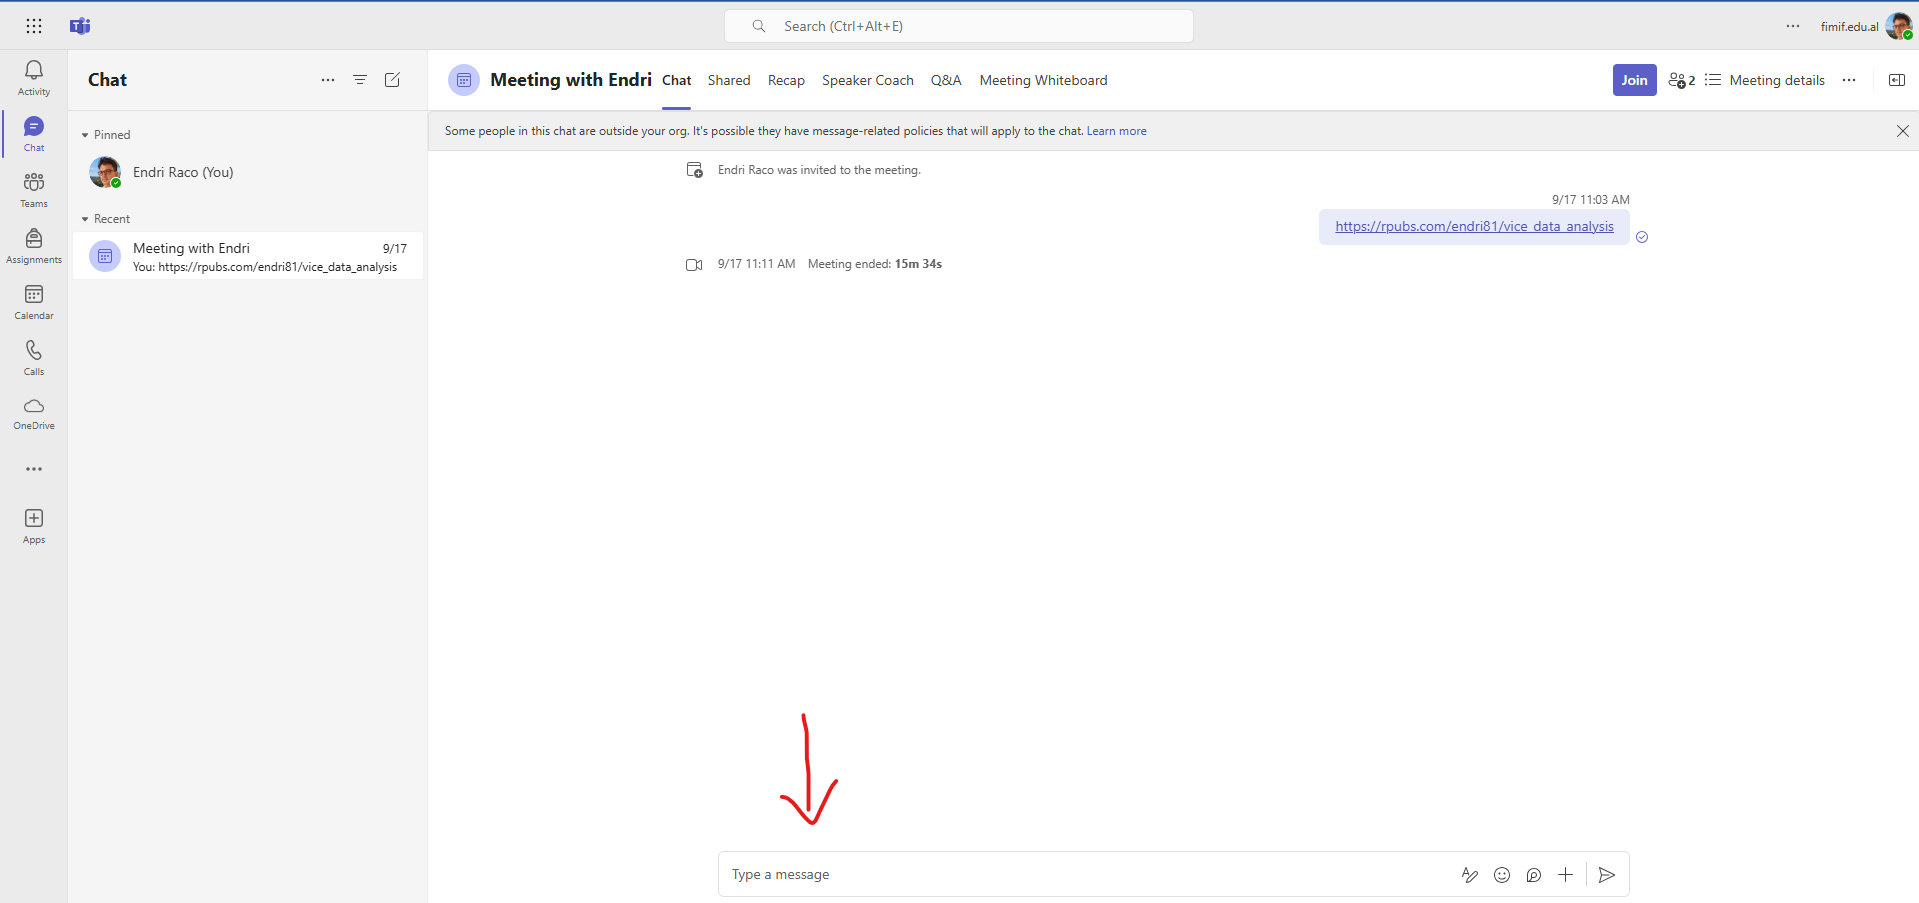
\includegraphics{./images/teams3.png}
\end{frame}

\begin{frame}{Organizimi i një takimi virtual}
\phantomsection\label{organizimi-i-njuxeb-takimi-virtual}
\begin{enumerate}
\tightlist
\item
  Klikoni mbi seksionin \textbf{Calendar}.
\end{enumerate}

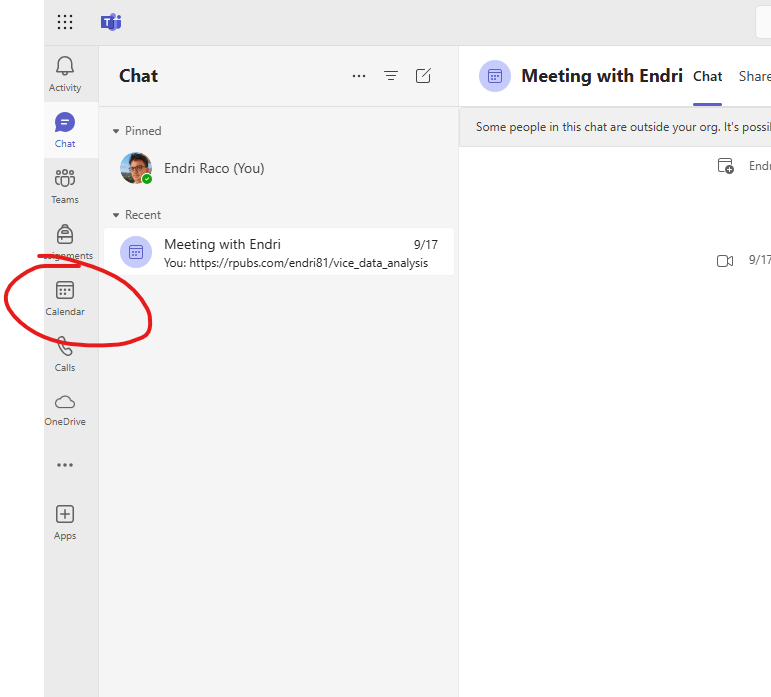
\includegraphics{./images/teams4.png}
\end{frame}

\begin{frame}{Organizimi i një takimi virtual}
\phantomsection\label{organizimi-i-njuxeb-takimi-virtual-1}
\begin{enumerate}
\setcounter{enumi}{1}
\tightlist
\item
  Zgjidhni \textbf{``New Meeting''} (Takim i Ri).
\end{enumerate}

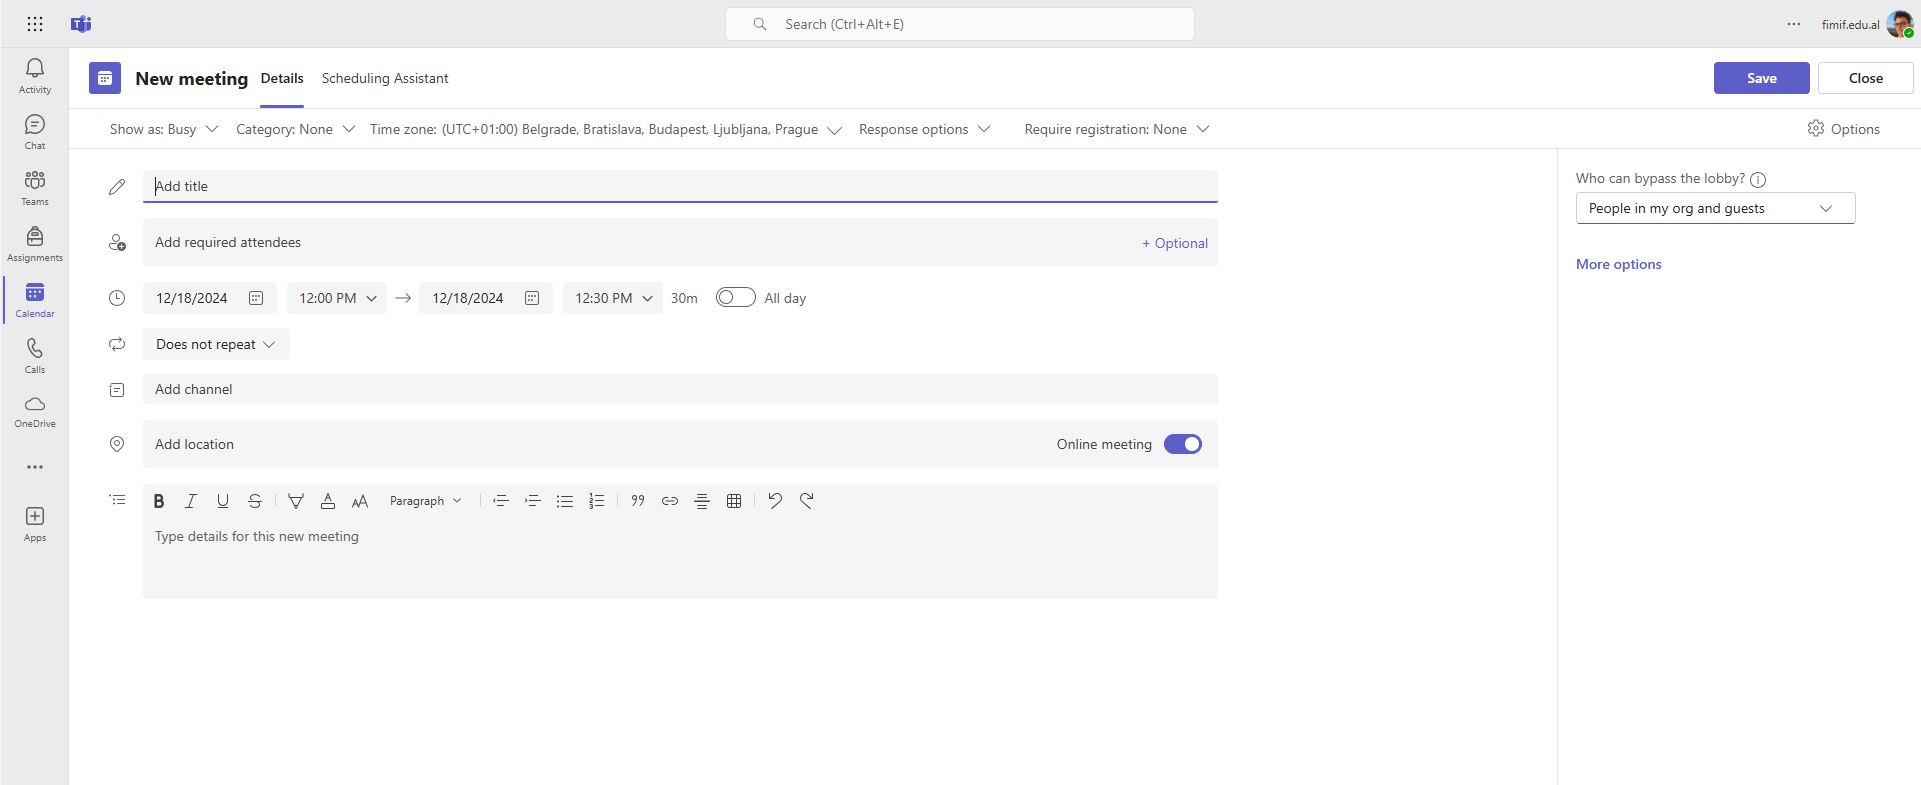
\includegraphics{./images/teams5.png}
\end{frame}

\begin{frame}{Organizimi i një takimi virtual}
\phantomsection\label{organizimi-i-njuxeb-takimi-virtual-2}
\begin{enumerate}
\setcounter{enumi}{2}
\item
  Plotësoni detajet:

  \begin{itemize}
  \item
    \textbf{Titulli} i takimit
  \item
    \textbf{Koha dhe data}
  \item
    \textbf{Pjesëmarrësit}
  \end{itemize}
\end{enumerate}
\end{frame}

\begin{frame}{Organizimi i një takimi virtual}
\phantomsection\label{organizimi-i-njuxeb-takimi-virtual-3}
\begin{enumerate}
\setcounter{enumi}{3}
\tightlist
\item
  Klikoni \textbf{``Save''} për të dërguar ftesat.
\end{enumerate}
\end{frame}

\begin{frame}{Rezultate}
\phantomsection\label{rezultate-5}
\begin{itemize}
\item
  \textbf{Microsoft Teams} është mjeti ideal për komunikim dhe
  bashkëpunim në kohë reale.
\item
  Mund të përdoret për:

  \begin{itemize}
  \item
    Planifikim takimesh.
  \item
    Bashkëpunim në projekte.
  \item
    Organizim të komunikimit në ekipe të strukturuara.
  \end{itemize}
\end{itemize}
\end{frame}

\begin{frame}{Pyetje \& Diskutim}
\phantomsection\label{pyetje-diskutim-8}
\begin{itemize}
\tightlist
\item
  A keni përdorur më parë \textbf{Microsoft Teams}?
\end{itemize}
\end{frame}

\begin{frame}{Bashkimi në një takim}
\phantomsection\label{bashkimi-nuxeb-njuxeb-takim}
\begin{enumerate}
\item
  Për t'u bashkuar në takim:

  \begin{itemize}
  \item
    Shkoni te \textbf{Calendar}.
  \item
    Klikoni mbi takimin dhe zgjidhni \textbf{``Join''} (Bashkohu).
  \end{itemize}
\end{enumerate}
\end{frame}

\begin{frame}{Bashkimi në një takim}
\phantomsection\label{bashkimi-nuxeb-njuxeb-takim-1}
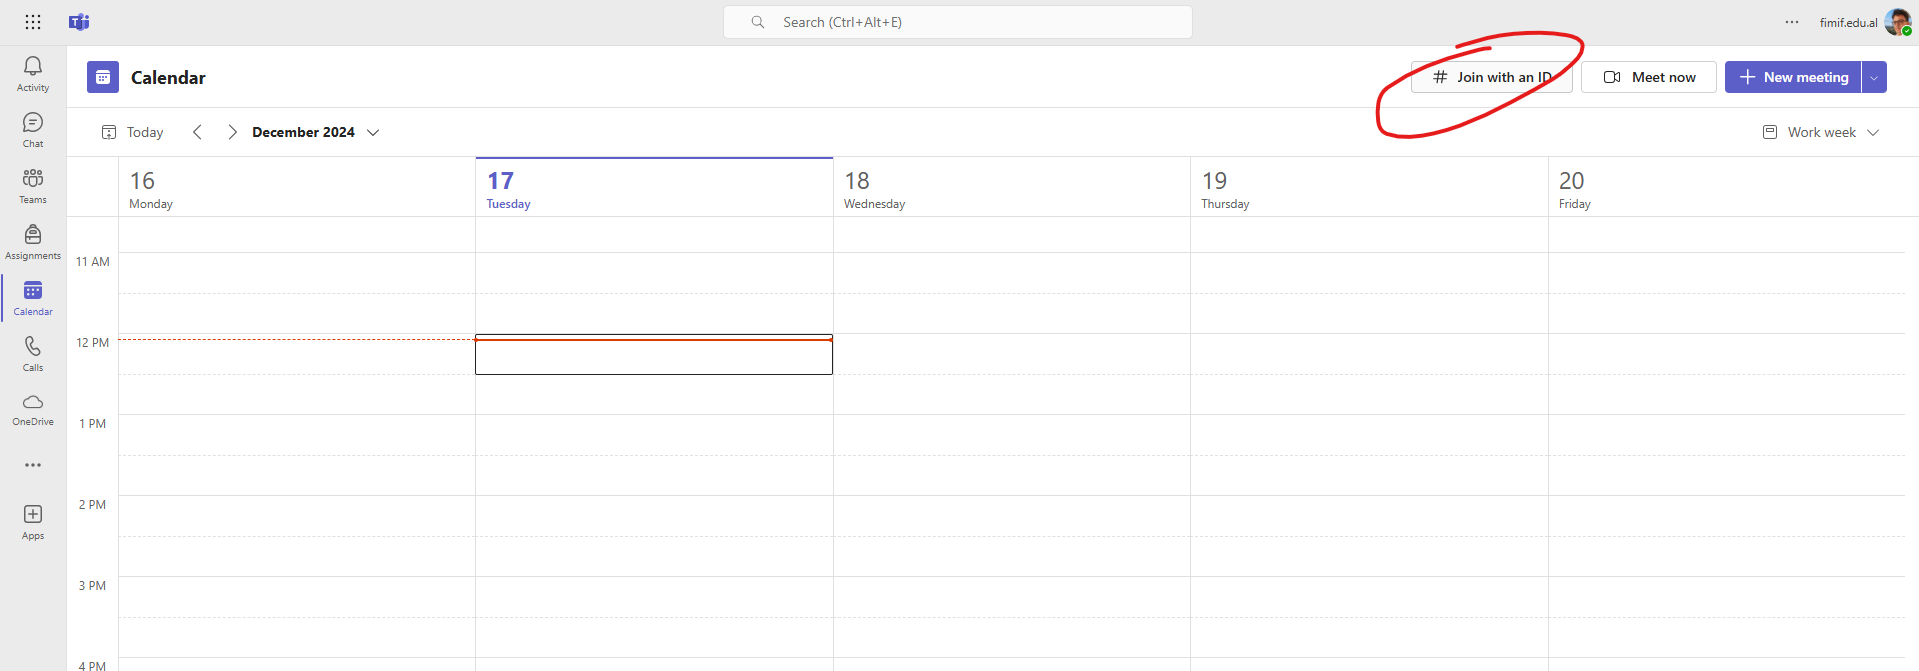
\includegraphics{./images/teams6.png}
\end{frame}

\begin{frame}{Bashkimi në një takim}
\phantomsection\label{bashkimi-nuxeb-njuxeb-takim-2}
\begin{enumerate}
\setcounter{enumi}{1}
\item
  Përshtasni opsionet përpara hyrjes:

  \begin{itemize}
  \tightlist
  \item
    Aktivizoni ose çaktivizoni \textbf{kamerën} dhe \textbf{mikrofonin}.
  \end{itemize}
\end{enumerate}

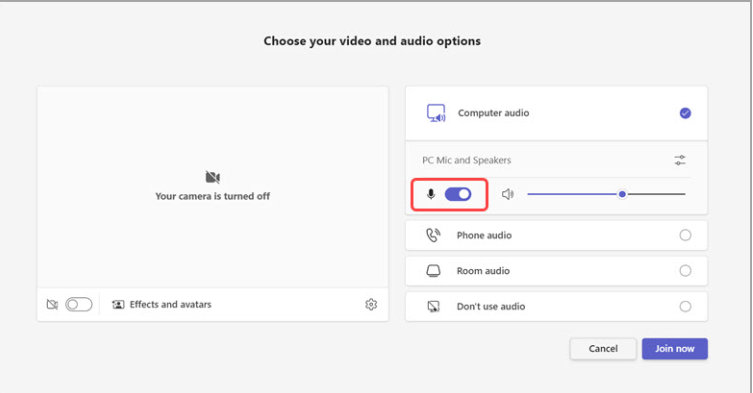
\includegraphics{./images/teams7.png}
\end{frame}

\begin{frame}{Shiriti i kontrolleve në takime}
\phantomsection\label{shiriti-i-kontrolleve-nuxeb-takime}
\begin{enumerate}
\item
  Kontrolli i takimeve ndodhet \textbf{në krye të ekranit}.
\item
  Ai përfshin funksione si:

  \begin{itemize}
  \tightlist
  \item
    \textbf{Chat}, \textbf{Participants}, \textbf{Raise hand},
    \textbf{React}, \textbf{Share}, dhe më shumë.
  \end{itemize}
\end{enumerate}

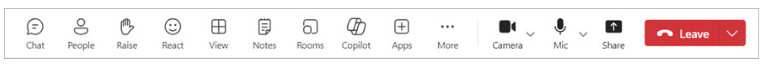
\includegraphics{./images/teams8.png}
\end{frame}

\begin{frame}{Shfaqja ose fshehja e bisedës (Chat)}
\phantomsection\label{shfaqja-ose-fshehja-e-biseduxebs-chat}
\begin{itemize}
\item
  Klikoni mbi ikonën \textbf{Chat} për të hapur bisedën e takimit.
\item
  Shkruani mesazhe për të komunikuar pa ndërprerë folësin.
\end{itemize}

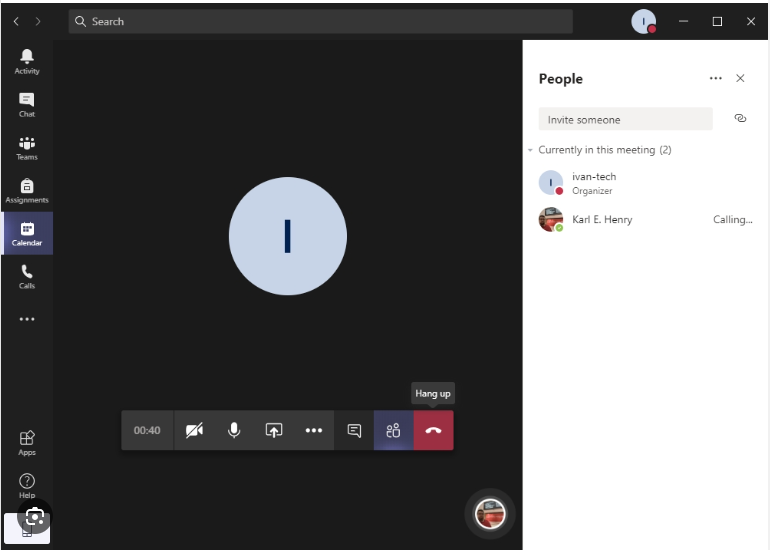
\includegraphics{./images/teams9.png}
\end{frame}

\begin{frame}{Shfaqja ose fshehja e bisedës (Chat)}
\phantomsection\label{shfaqja-ose-fshehja-e-biseduxebs-chat-1}
\begin{itemize}
\tightlist
\item
  Klikoni sërish për ta fshehur bisedën.
\end{itemize}
\end{frame}

\begin{frame}{Shfaqja ose fshehja e pjesëmarrësve}
\phantomsection\label{shfaqja-ose-fshehja-e-pjesuxebmarruxebsve}
\begin{itemize}
\item
  Klikoni mbi \textbf{Participants} për të parë listën e pjesëmarrësve.
\item
  Mund të:

  \begin{itemize}
  \tightlist
  \item
    \textbf{Ftoni persona të rinj} në takim.\\
  \item
    \textbf{Kontrolloni statusin} e pjesëmarrësve.
  \end{itemize}
\end{itemize}
\end{frame}

\begin{frame}{Shfaqja ose fshehja e pjesëmarrësve}
\phantomsection\label{shfaqja-ose-fshehja-e-pjesuxebmarruxebsve-1}
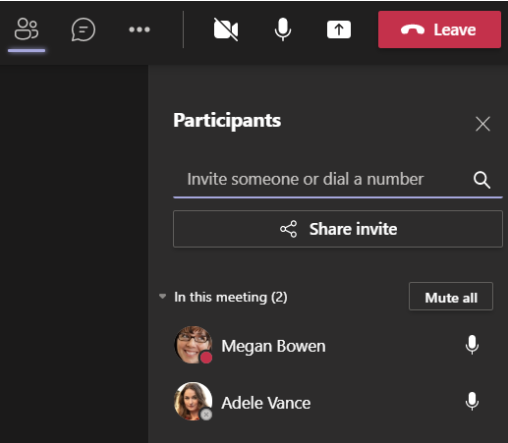
\includegraphics{./images/teams10.png}
\end{frame}

\begin{frame}{Ngitja e dorës (Raise Hand)}
\phantomsection\label{ngitja-e-doruxebs-raise-hand}
\begin{itemize}
\item
  Klikoni mbi ikonën \textbf{Raise Hand} për të ngritur dorën
  virtualisht.
\item
  Kjo i tregon folësit që dëshironi të flisni pa e ndërprerë atë.
\end{itemize}

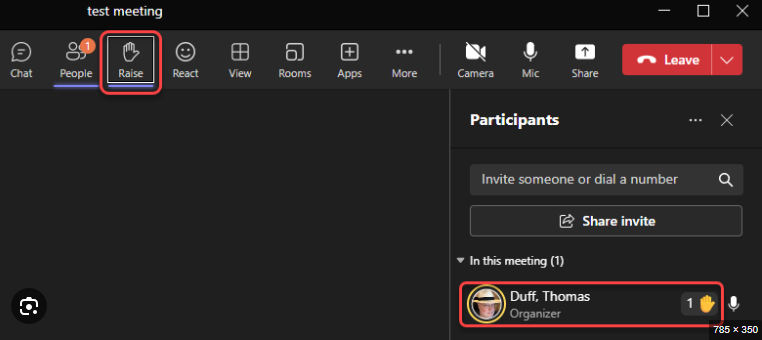
\includegraphics{./images/teams11.png}
\end{frame}

\begin{frame}{Ngitja e dorës (Raise Hand)}
\phantomsection\label{ngitja-e-doruxebs-raise-hand-1}
\begin{itemize}
\tightlist
\item
  Klikoni sërish për të ulur dorën.
\end{itemize}
\end{frame}

\begin{frame}{Shprehja e reagimeve (React)}
\phantomsection\label{shprehja-e-reagimeve-react}
\begin{itemize}
\item
  Klikoni mbi ikonën \textbf{React} për të zgjedhur një emoji reagim.
\item
  Reagimet shfaqen për disa sekonda në ekran për të gjithë
  pjesëmarrësit.
\end{itemize}

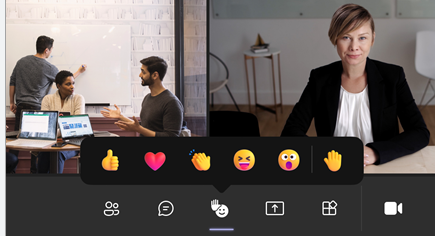
\includegraphics{./images/teams12.png}
\end{frame}

\begin{frame}{Ndarja e ekranit (Share)}
\phantomsection\label{ndarja-e-ekranit-share}
\begin{itemize}
\tightlist
\item
  Klikoni mbi \textbf{Share} për të ndarë përmbajtje:
\end{itemize}

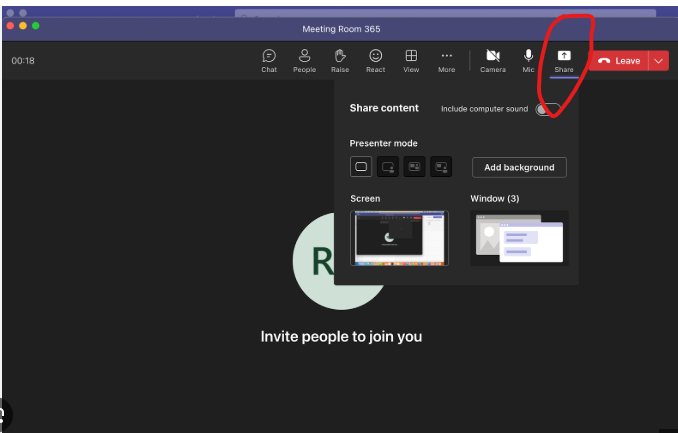
\includegraphics{./images/teams13.png}
\end{frame}

\begin{frame}{Ndarja e ekranit (Share)}
\phantomsection\label{ndarja-e-ekranit-share-1}
\begin{itemize}
\item
  \textbf{Entire screen} (Ekrani i plotë).
\item
  \textbf{Window} (Një aplikacion specifik).
\item
  \textbf{PowerPoint} ose \textbf{Whiteboard}.
\end{itemize}
\end{frame}

\begin{frame}{Ndryshimi i pamjes së takimit (View)}
\phantomsection\label{ndryshimi-i-pamjes-suxeb-takimit-view}
\begin{itemize}
\item
  Klikoni mbi ikonën \textbf{View} për të ndryshuar pamjen e
  pjesëmarrësve:

  \begin{itemize}
  \item
    \textbf{Gallery}: Pamje standarde me të gjithë pjesëmarrësit.
  \item
    \textbf{Together Mode}: Të gjithë pjesëmarrësit shfaqen në një
    ambient të përbashkët.
  \end{itemize}
\end{itemize}


\includegraphics{./images/teams14.png}
\end{frame}

\begin{frame}{Përdorimi i më shumë opsioneve (More Actions)}
\phantomsection\label{puxebrdorimi-i-muxeb-shumuxeb-opsioneve-more-actions}
\begin{itemize}
\item
  Klikoni mbi ikonën \textbf{More Actions} (\ldots) për të përdorur
  funksione shtesë:

  \begin{itemize}
  \item
    \textbf{Start Recording} (Fillo regjistrimin).
  \item
    \textbf{Turn off incoming video} (Fik pamjet e videove të tjera).
  \item
    \textbf{Apply background effects} (Ndrysho sfondin virtual).
  \end{itemize}
\end{itemize}
\end{frame}

\begin{frame}{Përdorimi i më shumë opsioneve (More Actions)}
\phantomsection\label{puxebrdorimi-i-muxeb-shumuxeb-opsioneve-more-actions-1}
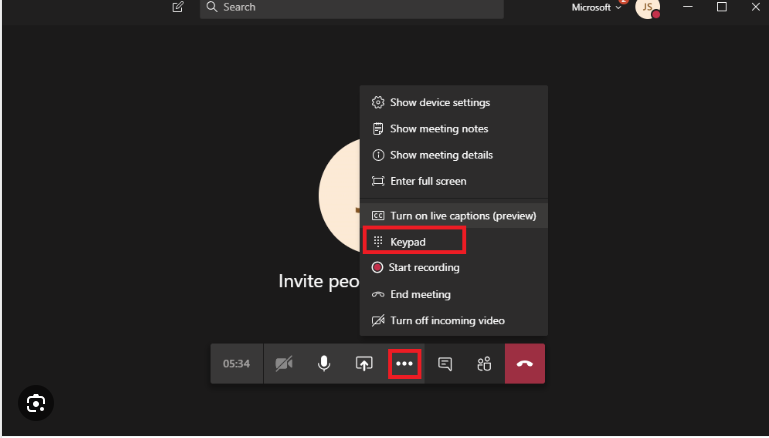
\includegraphics{./images/teams15.png}
\end{frame}

\begin{frame}{Regjistrimi i takimit}
\phantomsection\label{regjistrimi-i-takimit}
\begin{itemize}
\item
  Klikoni \textbf{Start Recording} për të regjistruar takimin.
\item
  Regjistrimi ruhet automatikisht në \textbf{OneDrive} ose
  \textbf{SharePoint}.
\end{itemize}

\includegraphics{./images/teams16.png}
\end{frame}

\begin{frame}{Aktivizimi ose çaktivizimi i mikrofonit dhe kamerës}
\phantomsection\label{aktivizimi-ose-uxe7aktivizimi-i-mikrofonit-dhe-kameruxebs}
\begin{itemize}
\item
  Klikoni mbi \textbf{Mic} për të ndërruar midis muting/unmuting.
\item
  Klikoni mbi \textbf{Camera} për të aktivizuar ose çaktivizuar videon.
\end{itemize}
\end{frame}

\begin{frame}{Aktivizimi ose çaktivizimi i mikrofonit dhe kamerës}
\phantomsection\label{aktivizimi-ose-uxe7aktivizimi-i-mikrofonit-dhe-kameruxebs-1}
\begin{itemize}
\tightlist
\item
  Përdorni shigjetën pranë ikonave për të modifikuar cilësimet.
\end{itemize}

\includegraphics{./images/teams17.png}
\end{frame}

\begin{frame}{Dalja nga takimi}
\phantomsection\label{dalja-nga-takimi}
\begin{itemize}
\item
  Klikoni mbi \textbf{Leave} (Largohu) për të dalë nga takimi.
\item
  Nëse jeni organizatori, mund të zgjidhni \textbf{End Meeting} për të
  mbyllur takimin për të gjithë.
\end{itemize}

\includegraphics{./images/teams18.png}
\end{frame}

\begin{frame}{Përfitimet e përdorimit të kontrolleve të Teams}
\phantomsection\label{puxebrfitimet-e-puxebrdorimit-tuxeb-kontrolleve-tuxeb-teams}
\begin{enumerate}
\item
  \textbf{Komunikim i qartë}: Biseda dhe reagime pa ndërprerje.
\item
  \textbf{Menaxhim më i mirë}: Kontroll i pjesëmarrësve dhe
  regjistrimeve.
\item
  \textbf{Bashkëpunim i përmirësuar}: Ndarja e ekranit dhe pamje të
  personalizuara.
\end{enumerate}
\end{frame}

\begin{frame}{Rezultate}
\phantomsection\label{rezultate-6}
\begin{itemize}
\item
  Përdorimi i kontrolleve të Microsoft Teams siguron që takimet të jenë
  \textbf{efektive} dhe \textbf{produktive}.
\item
  Eksploroni funksionalitetet për të përmirësuar bashkëpunimin tuaj
  gjatë takimeve.
\end{itemize}
\end{frame}

\begin{frame}{Pyetje \& Diskutim}
\phantomsection\label{pyetje-diskutim-9}
\begin{itemize}
\tightlist
\item
  A ka ndonjë funksion specifik që dëshironi të eksploroni më thellë?
\end{itemize}
\end{frame}

\section{Microsoft OneDrive}\label{microsoft-onedrive}

\begin{frame}{Microsoft OneDrive}
\phantomsection\label{microsoft-onedrive-1}
\begin{itemize}
\item
  \textbf{Microsoft OneDrive} është një shërbim ruajtjeje cloud në
  \textbf{Office 365}.
\item
  Ju mund të:

  \begin{itemize}
  \item
    Ruani dokumente dhe skedarë në mënyrë të sigurt.
  \item
    Aksesohet nga \textbf{çdo pajisje} përmes një shfletuesi web.
  \item
    Ndani dhe bashkëpunoni në kohë reale me kolegë dhe miq.
  \end{itemize}
\end{itemize}
\end{frame}

\begin{frame}{Hapja e OneDrive nga paneli kryesor}
\phantomsection\label{hapja-e-onedrive-nga-paneli-kryesor}
\begin{enumerate}
\item
  Pasi të jeni identifikuar, do të shfaqet \textbf{paneli kryesor} i
  Office 365.
\item
  Klikoni mbi ikonën \textbf{OneDrive} (ikonë blu me një re të bardhë).
\end{enumerate}

\includegraphics{./images/onedrive1.png}
\end{frame}

\begin{frame}{Ndërfaqja e OneDrive Web}
\phantomsection\label{nduxebrfaqja-e-onedrive-web}
\begin{enumerate}
\item
  Pas hapjes së OneDrive, do të shihni ndërfaqen kryesore:

  \begin{itemize}
  \item
    \textbf{My Files} (Skedarët e mi): Skedarët dhe dosjet tuaja.
  \item
    \textbf{Recent} (Së fundmi): Dokumentet e aksesuar kohët e fundit.
  \item
    \textbf{Shared} (Të ndara): Dokumentet që keni ndarë ose ju janë
    ndarë.
  \end{itemize}
\end{enumerate}
\end{frame}

\begin{frame}{Ndërfaqja e OneDrive Web}
\phantomsection\label{nduxebrfaqja-e-onedrive-web-1}
\includegraphics{./images/onedrive2.png}
\end{frame}

\begin{frame}{Ngarkimi i skedarëve në OneDrive}
\phantomsection\label{ngarkimi-i-skedaruxebve-nuxeb-onedrive}
\begin{enumerate}
\item
  Klikoni mbi butonin \textbf{``Upload''} (Ngarko) në krye të ekranit.
\item
  Zgjidhni:

  \begin{itemize}
  \item
    \textbf{Files} (Skedarë): Për të ngarkuar një ose më shumë skedarë.
  \item
    \textbf{Folder} (Dosje): Për të ngarkuar një dosje të tërë.
  \end{itemize}
\end{enumerate}
\end{frame}

\begin{frame}{Ngarkimi i skedarëve në OneDrive}
\phantomsection\label{ngarkimi-i-skedaruxebve-nuxeb-onedrive-1}
\begin{enumerate}
\setcounter{enumi}{2}
\tightlist
\item
  Zgjidhni skedarët ose dosjet nga kompjuteri juaj.
\end{enumerate}

\includegraphics{./images/onedrive3.png}
\end{frame}

\begin{frame}{Krijimi i dokumenteve të rinj në OneDrive}
\phantomsection\label{krijimi-i-dokumenteve-tuxeb-rinj-nuxeb-onedrive}
\begin{enumerate}
\item
  Klikoni butonin \textbf{``New''} në krye të ekranit.
\item
  Zgjidhni llojin e dokumentit që dëshironi të krijoni:

  \begin{itemize}
  \tightlist
  \item
    \textbf{Word}, \textbf{Excel}, \textbf{PowerPoint}, \textbf{OneNote}
    ose \textbf{Folder}.
  \end{itemize}
\end{enumerate}
\end{frame}

\begin{frame}{Krijimi i dokumenteve të rinj në OneDrive}
\phantomsection\label{krijimi-i-dokumenteve-tuxeb-rinj-nuxeb-onedrive-1}
\begin{enumerate}
\setcounter{enumi}{2}
\tightlist
\item
  Dokumenti i ri do të hapet automatikisht në versionin online.
\end{enumerate}

\includegraphics{./images/onedrive4.png}
\end{frame}

\begin{frame}{Hapja dhe organizimi i skedarëve}
\phantomsection\label{hapja-dhe-organizimi-i-skedaruxebve}
\begin{enumerate}
\item
  Klikoni mbi një skedar për ta \textbf{hapur} ose \textbf{redaktuar}.
\item
  Për të organizuar skedarët:

  \begin{itemize}
  \item
    Klikoni me të djathtën mbi një skedar për të:

    \begin{itemize}
    \item
      \textbf{Rename} (Riemërtuar).
    \item
      \textbf{Move to} (Zhvendosur në dosje).
    \item
      \textbf{Delete} (Fshirë).
    \end{itemize}
  \end{itemize}
\end{enumerate}
\end{frame}

\begin{frame}{Hapja dhe organizimi i skedarëve}
\phantomsection\label{hapja-dhe-organizimi-i-skedaruxebve-1}
\includegraphics{./images/onedrive5.png}
\end{frame}

\begin{frame}{Ndani skedarët me të tjerët}
\phantomsection\label{ndani-skedaruxebt-me-tuxeb-tjeruxebt}
\begin{enumerate}
\item
  Zgjidhni skedarin që dëshironi të ndani.
\item
  Klikoni mbi butonin \textbf{``Share''} (Ndaj) në krye të ekranit.
\end{enumerate}
\end{frame}

\begin{frame}{Ndani skedarët me të tjerët}
\phantomsection\label{ndani-skedaruxebt-me-tuxeb-tjeruxebt-1}
\includegraphics{./images/onedrive5.png}
\end{frame}

\begin{frame}{Ndani skedarët me të tjerët}
\phantomsection\label{ndani-skedaruxebt-me-tuxeb-tjeruxebt-2}
\begin{enumerate}
\setcounter{enumi}{2}
\item
  Zgjidhni mënyrën e ndarjes:

  \begin{itemize}
  \item
    Futni adresën e email-it të personit.
  \item
    Vendosni lejet (p.sh., \textbf{View only} ose \textbf{Edit}).
  \end{itemize}
\item
  Klikoni \textbf{Send} për të ndarë skedarin.
\end{enumerate}
\end{frame}

\begin{frame}{Aksesi nga çdo pajisje}
\phantomsection\label{aksesi-nga-uxe7do-pajisje}
\begin{itemize}
\item
  Për të aksesuar OneDrive nga pajisje të tjera:

  \begin{itemize}
  \item
    Shkoni te \textbf{\url{https://onedrive.live.com}}.
  \item
    Identifikohuni me të njëjtat kredenciale.
  \end{itemize}
\item
  OneDrive mund të përdoret edhe përmes \textbf{aplikacionit mobile} për
  Android dhe iOS.
\end{itemize}
\end{frame}

\begin{frame}{Përfitimet e përdorimit të OneDrive}
\phantomsection\label{puxebrfitimet-e-puxebrdorimit-tuxeb-onedrive}
\begin{itemize}
\item
  \textbf{Ruajtje në cloud}: Skedarët tuaj janë gjithmonë të sigurt dhe
  të aksesueshëm.
\item
  \textbf{Bashkëpunim}: Ndani dhe redaktoni dokumente me kolegët në kohë
  reale.
\item
  \textbf{Akses i lehtë}: Aksesohet nga çdo pajisje me një lidhje
  interneti.
\item
  \textbf{Siguri}: Skedarët janë të mbrojtur dhe të enkriptuar nga
  Microsoft.
\end{itemize}
\end{frame}

\begin{frame}{Rezultate}
\phantomsection\label{rezultate-7}
\begin{itemize}
\item
  \textbf{Microsoft OneDrive} ju lejon të ruani, organizoni dhe ndani
  skedarët tuaj me lehtësi.
\item
  Aksesi përmes shfletuesit është i thjeshtë dhe nuk kërkon instalim
  softueri.
\item
  Përdorni funksionet \textbf{Upload}, \textbf{Share}, dhe \textbf{Edit}
  për të maksimizuar përfitimet e OneDrive.
\end{itemize}
\end{frame}

\begin{frame}{Pyetje \& Diskutim}
\phantomsection\label{pyetje-diskutim-10}
\begin{itemize}
\tightlist
\item
  A keni përdorur më parë OneDrive për ruajtjen e skedarëve?
\end{itemize}
\end{frame}

\end{document}
